\documentclass[11pt]{article}

\usepackage[letterpaper,margin=0.95in]{geometry}
\usepackage{graphicx}
\usepackage{booktabs}
\usepackage{amsmath}
\usepackage{amssymb}
\usepackage{xcolor}
\usepackage{caption}
\usepackage{enumitem}
\usepackage[T1]{fontenc}
\usepackage{lmodern}
\usepackage{tikz}
\usepackage{pgfplots}
\usepackage{titlesec}
\usepackage[colorlinks=true,linkcolor=accent,citecolor=black,urlcolor=accent]{hyperref}

\pgfplotsset{compat=1.18}
\usetikzlibrary{positioning,arrows.meta,fit,backgrounds,calc,shapes.geometric,
                decorations.pathreplacing,patterns,shadows.blur}

% ---------------------------------------------------------------- palette
\definecolor{ink}{HTML}{1A1A1A}
\definecolor{ink2}{HTML}{555555}
\definecolor{muted}{HTML}{8A8A8A}
\definecolor{accent}{HTML}{1F6FEB}
\definecolor{accentbg}{HTML}{E7F0FD}
\definecolor{bad}{HTML}{D1242F}
\definecolor{badbg}{HTML}{FFEBE9}
\definecolor{good}{HTML}{1A7F37}
\definecolor{goodbg}{HTML}{E6F4EA}
\definecolor{warn}{HTML}{BF8700}
\definecolor{warnbg}{HTML}{FFF8C5}
\definecolor{rule}{HTML}{D8DEE4}
\definecolor{shade}{HTML}{F6F8FA}

\captionsetup{font=small,labelfont=bf,labelsep=period}
\setlist{itemsep=2pt,topsep=4pt,parsep=0pt}
\emergencystretch=3em
\widowpenalty=300
\clubpenalty=300
\sloppy
\hyphenpenalty=400

\titleformat{\section}{\Large\bfseries\color{ink}}{\thesection.}{0.5em}{}
\titleformat{\subsection}{\large\bfseries\color{ink}}{\thesubsection}{0.6em}{}
\titlespacing{\section}{0pt}{1.6em}{0.7em}
\titlespacing{\subsection}{0pt}{1.1em}{0.4em}

% ---------------------------------------------------------------- shorthands
\newcommand{\f}[1]{\textcolor{accent}{\texttt{#1}}}
\newcommand{\code}[1]{\texttt{\small #1}}
\newcommand{\wg}{worst-group}

% a labelled callout box
\newenvironment{note}[2]{%
  \par\medskip\noindent
  \begin{tikzpicture}
  \node[draw=#1,fill=#1!8,line width=0.9pt,rounded corners=3pt,
        inner sep=8pt,text width=0.955\textwidth,align=left,font=\small] (b) \bgroup
  \textcolor{#1}{\bfseries #2}\par\smallskip
}{%
  \egroup;
  \end{tikzpicture}\par\medskip
}

% ---------------------------------------------------------------- tikz styles
\tikzset{
  blk/.style={draw=rule,line width=0.9pt,fill=white,rounded corners=3pt,
              align=center,font=\small,inner sep=6pt,minimum height=9mm},
  blkf/.style={blk,fill=shade},
  blka/.style={blk,draw=accent,fill=accentbg},
  blkb/.style={blk,draw=bad,fill=badbg},
  blkg/.style={blk,draw=good,fill=goodbg},
  blkw/.style={blk,draw=warn,fill=warnbg},
  lbl/.style={font=\scriptsize\itshape,text=ink2},
  tiny/.style={font=\scriptsize,text=ink2},
  ar/.style={-{Stealth[length=5pt,width=4pt]},draw=ink2,line width=0.9pt},
  arb/.style={ar,draw=bad},
  arg/.style={ar,draw=good},
  cell/.style={draw=rule,line width=0.8pt,minimum width=34mm,minimum height=15mm,
               align=center,font=\small},
}

\raggedbottom

\begin{document}

% ================================================================ TITLE
\thispagestyle{empty}
\begin{center}
\vspace*{0.3in}
{\Huge\bfseries Understanding this project}\\[0.9em]
{\large Compression vs.\ group robustness on Waterbirds}\\[1.6em]
{\color{ink2}\large A plain-English tour of the idea and every file in the repo}\\[2.2em]
\end{center}

\begin{center}
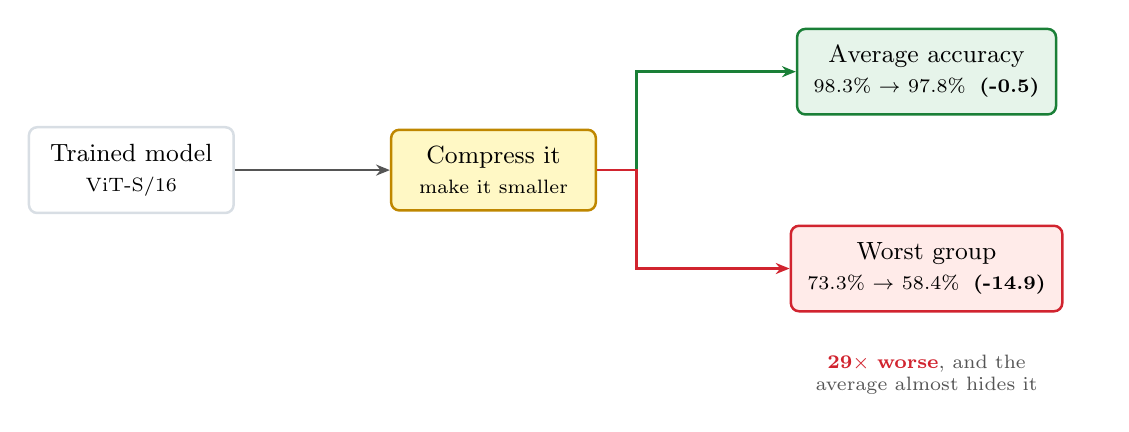
\begin{tikzpicture}[scale=1.0]
% the one-picture version of the whole project
\node[blk,minimum width=26mm] (model) at (0,0) {Trained model\\\scriptsize ViT-S/16};
\node[blkw,minimum width=26mm] (comp) at (4.6,0) {Compress it\\\scriptsize make it smaller};
\draw[ar] (model) -- (comp);

\node[blkg,minimum width=30mm,align=center] (avg) at (10.1,1.25)
  {Average accuracy\\\scriptsize 98.3\% $\to$ 97.8\% \;\textbf{(-0.5)}};
\node[blkb,minimum width=30mm,align=center] (wgn) at (10.1,-1.25)
  {Worst group\\\scriptsize 73.3\% $\to$ 58.4\% \;\textbf{(-14.9)}};
\draw[arg] (comp.east) -- ++(0.5,0) |- (avg.west);
\draw[arb] (comp.east) -- ++(0.5,0) |- (wgn.west);

\node[tiny,text width=42mm,align=center] at (10.1,-2.6)
  {\textcolor{bad}{\bfseries 29$\times$ worse}, and the\\average almost hides it};
\end{tikzpicture}
\end{center}

\vfill
\begin{center}
{\color{ink2}\small
Everything in here was checked against the actual files in the repo.\\
Every number is an average over \textbf{3 training runs} (seeds 0, 1, 2), from
\code{results/sweep.csv},\\ \code{results/sweep\_spur*.csv} and
\code{results/retention\_*.csv}. Both phases have been run.}
\end{center}
\vspace{0.4in}
\clearpage

\tableofcontents
\clearpage

% ================================================================ PART 0
\section{The 60-second version}

Here's the whole project in one breath:

\begin{note}{accent}{The question}
You train a model. It works. Then you shrink it so it's cheaper to run --
everyone does this before shipping. \textbf{Does shrinking it quietly break the
groups it was already bad at?}
\end{note}

\noindent And the answer we got: \textbf{yes, and if you only look at average
accuracy you'd never notice.}

Chop 30\% of the weights out of our model and average accuracy drops by
\textbf{0.5 points}. Sounds free. But the worst-performing group of images drops
by \textbf{14.9 points}. That's about 29 times bigger. Report only the average
and you'd call that compression free, ship it, and the model would be
meaningfully worse for exactly the cases it already struggled with.

It gets sharper. Delete 6 attention heads out of 72 -- that's 2.8\% of the
weights we're allowed to touch -- and the average loses 1.7 points while the
worst group loses \textbf{18.2}.

And then we asked the obvious follow-up: what if you \emph{fix} the robustness
problem first, and only then compress? The short answer is that the fix works
(worst group goes from 73.3\% to \textbf{87.9\%}), it \emph{does} survive gentle
compression, and it stops surviving at exactly the point where compression has
broken the model for everyone. Section~\ref{sec:phase2} has the numbers.

\subsection*{The three words you need}

\begin{itemize}[leftmargin=1.4em]
\item \textbf{Shortcut.} Our dataset is birds. Water birds are usually
photographed on water, land birds on land. So the model learns ``water
background $=$ water bird'' instead of actually learning what a bird looks like.
It's lazy, and it works most of the time.

\item \textbf{Group.} Split the test set by (what bird it is) $\times$ (what
background it's on). Four groups. Two of them agree with the shortcut, two
fight it. The ones that fight it are where the model is weak.

\item \textbf{Worst-group accuracy.} Accuracy on the single worst of those four
groups. This is the number that actually tells you whether the model learned
birds or learned backgrounds.
\end{itemize}

\subsection*{What the repo does, start to finish}

\begin{center}
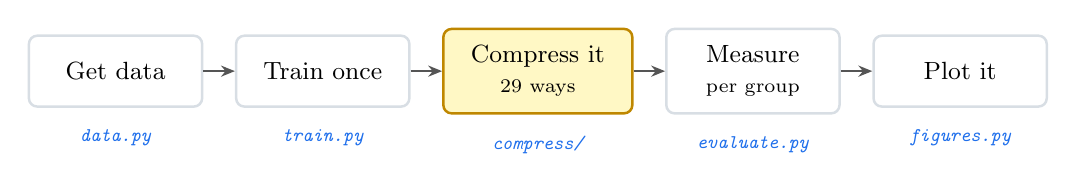
\begin{tikzpicture}[node distance=4mm]
\node[blk,minimum width=22mm] (d) {Get data};
\node[blk,minimum width=22mm,right=of d] (t) {Train once};
\node[blkw,minimum width=24mm,right=of t] (c) {Compress it\\\scriptsize 29 ways};
\node[blk,minimum width=22mm,right=of c] (e) {Measure\\\scriptsize per group};
\node[blk,minimum width=22mm,right=of e] (p) {Plot it};
\draw[ar] (d)--(t); \draw[ar] (t)--(c); \draw[ar] (c)--(e); \draw[ar] (e)--(p);
\node[lbl,below=1.5mm of d] {\f{data.py}};
\node[lbl,below=1.5mm of t] {\f{train.py}};
\node[lbl,below=1.5mm of c] {\f{compress/}};
\node[lbl,below=1.5mm of e] {\f{evaluate.py}};
\node[lbl,below=1.5mm of p] {\f{figures.py}};
\end{tikzpicture}
\end{center}

\noindent That's Phase 1. Phase 2 adds one step in front of it -- throw away
some training images first, then do the same thing -- and asks whether the fix
survives. Both phases are done. Section~\ref{sec:phase2} has the answers,
Section~\ref{sec:figures} explains how to read the pictures.


% ================================================================ PART 1
\section{The concepts, with zero code}

Skip this part if you already get shortcut learning. Otherwise this is the
foundation for everything else.

\subsection{The dataset: Waterbirds}

Waterbirds is a dataset built on purpose to be a trap. Someone took photos of
birds, cut the birds out, and pasted them onto new backgrounds. They controlled
exactly how often each bird type lands on each background type.

Here's what the training set looks like. Each box is a group, and the number is
how many training images are in it:

\begin{center}
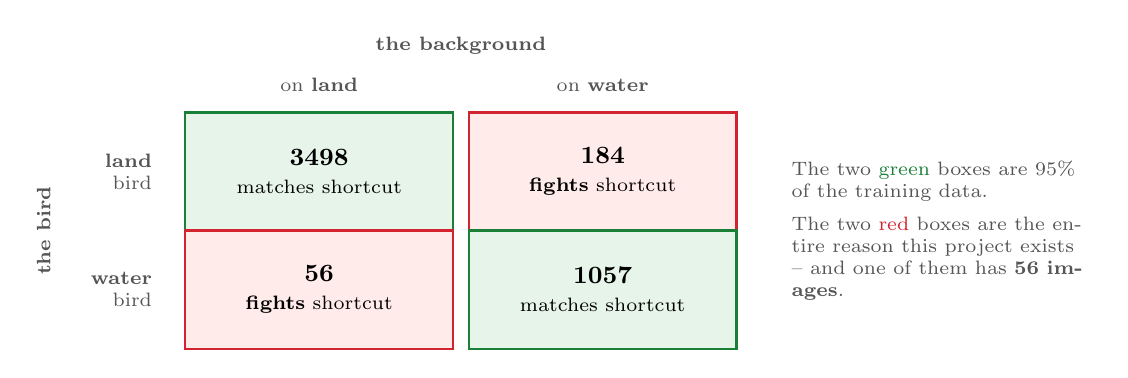
\begin{tikzpicture}
\node[tiny,rotate=90] at (-4.5,0.0) {\bfseries the bird};
\node[tiny] at (0.8,2.35) {\bfseries the background};

\node[tiny] at (-1.0,1.85) {on \textbf{land}};
\node[tiny] at (2.6,1.85) {on \textbf{water}};
\node[tiny,align=right,anchor=east] at (-3.0,0.75) {\textbf{land}\\bird};
\node[tiny,align=right,anchor=east] at (-3.0,-0.75) {\textbf{water}\\bird};

\node[cell,fill=goodbg,draw=good] at (-1.0,0.75) {\textbf{3498}\\[-1pt]\scriptsize matches shortcut};
\node[cell,fill=badbg,draw=bad]   at ( 2.6,0.75) {\textbf{184}\\[-1pt]\scriptsize \textbf{fights} shortcut};
\node[cell,fill=badbg,draw=bad]   at (-1.0,-0.75){\textbf{56}\\[-1pt]\scriptsize \textbf{fights} shortcut};
\node[cell,fill=goodbg,draw=good] at ( 2.6,-0.75){\textbf{1057}\\[-1pt]\scriptsize matches shortcut};

\node[tiny,text width=38mm,align=left] at (6.9,0.0)
  {The two \textcolor{good}{green} boxes are 95\% of the training data.\\[4pt]
   The two \textcolor{bad}{red} boxes are the entire reason this project exists
   -- and one of them has \textbf{56 images}.};
\end{tikzpicture}
\end{center}

\noindent Look at that imbalance. 3498 land birds on land, but only 56 water
birds on land. If you're a model trying to minimise your loss, you will notice
that ``is the background wet?'' predicts the label correctly 95\% of the time,
and that's a much easier thing to learn than bird anatomy.

\subsection{What the model actually learns}

\begin{center}
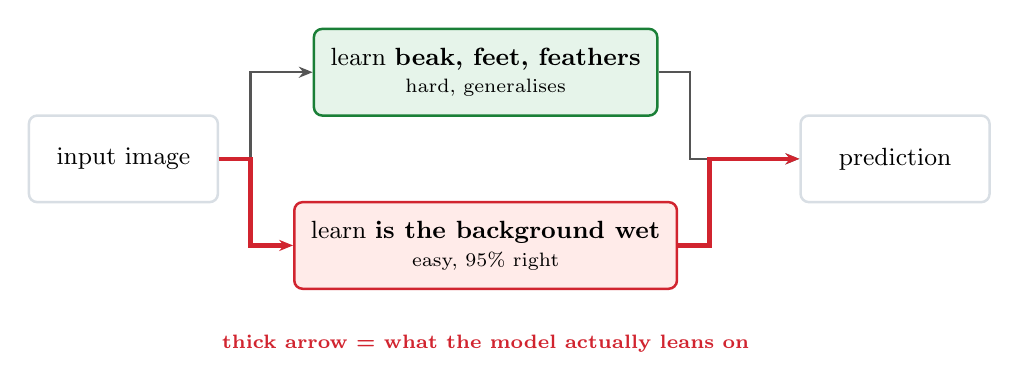
\begin{tikzpicture}
\node[blk,minimum width=24mm,minimum height=11mm] (img) at (0,0) {input image};

\node[blkg,minimum width=36mm,minimum height=11mm] (hard) at (4.6,1.1)
  {learn \textbf{beak, feet, feathers}\\[-1pt]\scriptsize hard, generalises};
\node[blkb,minimum width=36mm,minimum height=11mm] (easy) at (4.6,-1.1)
  {learn \textbf{is the background wet}\\[-1pt]\scriptsize easy, 95\% right};

\draw[ar] (img.east) -- ++(0.4,0) |- (hard.west);
\draw[arb,line width=1.6pt] (img.east) -- ++(0.4,0) |- (easy.west);

\node[blk,minimum width=24mm,minimum height=11mm] (out) at (9.8,0) {prediction};
\draw[ar] (hard.east) -- ++(0.4,0) |- (out.west);
\draw[arb,line width=1.6pt] (easy.east) -- ++(0.4,0) |- (out.west);

\node[tiny] at (4.6,-2.35) {\textcolor{bad}{\bfseries thick arrow = what the model actually leans on}};
\end{tikzpicture}
\end{center}

\noindent Nothing in plain training punishes the shortcut. It's not a bug in the
model, it's the rational move given the data. That's what makes it interesting.

\subsection{Why average accuracy lies}

Average accuracy lies to you. Our model scores 98.2\% and you'd think you're
done. But break it down by group:

\begin{center}
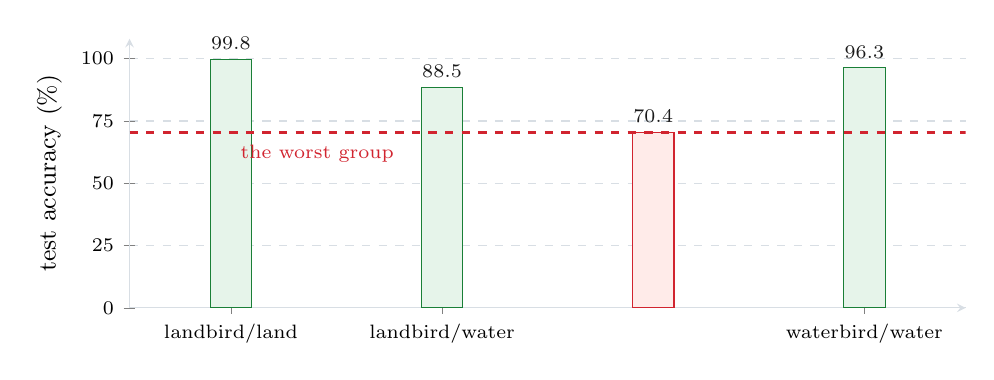
\begin{tikzpicture}
\begin{axis}[
  width=12.2cm, height=5.0cm,
  ybar, bar width=15pt,
  ymin=0, ymax=108,
  ylabel={test accuracy (\%)},
  ylabel style={font=\small},
  symbolic x coords={landbird/land,landbird/water,waterbird/land,waterbird/water},
  xtick=data, xticklabel style={font=\scriptsize},
  ytick={0,25,50,75,100}, yticklabel style={font=\scriptsize},
  nodes near coords, every node near coord/.append style={font=\scriptsize,color=ink},
  axis lines=left, axis line style={draw=rule},
  ymajorgrids, grid style={draw=rule,dashed},
  enlarge x limits=0.16,
]
\addplot[draw=good,fill=goodbg,bar shift=0pt] coordinates
  {(landbird/land,99.8) (landbird/water,88.5) (waterbird/water,96.3)};
\addplot[draw=bad,fill=badbg,bar shift=0pt] coordinates {(waterbird/land,70.4)};
\draw[dashed,bad,line width=1pt]
  ({rel axis cs:0,0}|-{axis cs:landbird/land,70.4}) -- ({rel axis cs:1,0}|-{axis cs:landbird/land,70.4});
\node[font=\scriptsize,bad,anchor=west] at (axis cs:landbird/land,62) {the worst group};
\end{axis}
\end{tikzpicture}
\end{center}

\noindent There it is. \textbf{99.8\%} on the easy group, \textbf{70.4\%} on
water birds photographed on land -- the group with 56 training images that
fights the shortcut. A 29-point spread, and the average buries it.

So we track three numbers, and you need to know the difference:

\begin{center}
\begin{tabular}{@{}lll@{}}
\toprule
\textbf{Number} & \textbf{On our model} & \textbf{What it means} \\
\midrule
plain average      & 91.7\% & straight mean over the test set \\
adjusted average   & 98.2\% & reweighted to match \emph{training} group frequencies \\
\textbf{worst group} & \textbf{70.4\%} & the single weakest group. the honest one \\
\bottomrule
\end{tabular}
\end{center}

\begin{note}{warn}{Why two different ``averages''?}
The test set is way more balanced than the training set (test is
2255/2255/642/642; training is 3498/184/56/1057). So a plain test average
over-weights the rare groups compared to how often they actually show up in
training. The \emph{adjusted} average reweights per-group accuracy by training
frequency, and that's the $\sim$98\% number everyone in this research area
quotes. We report it so our numbers are comparable to published work. The code
is \f{metrics.py}, function \code{adjusted\_average}.
\end{note}

\subsection{What ``compression'' means here}

Compression means making the model smaller or cheaper after it's already
trained. We try four flavours, and they're genuinely different operations:

\begin{center}
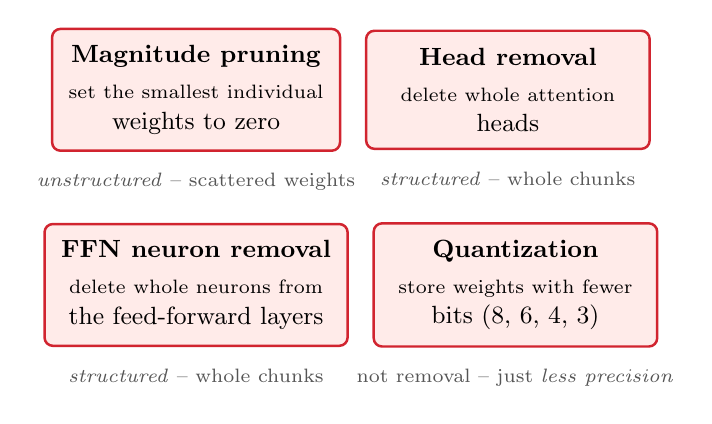
\begin{tikzpicture}[node distance=3mm]
\node[blkb,minimum width=36mm,minimum height=15mm,align=center] (m)
  {\textbf{Magnitude pruning}\\[2pt]\scriptsize set the smallest individual\\weights to zero};
\node[blkb,minimum width=36mm,minimum height=15mm,right=of m,align=center] (h)
  {\textbf{Head removal}\\[2pt]\scriptsize delete whole attention\\heads};
\node[blkb,minimum width=36mm,minimum height=15mm,below=9mm of m,align=center] (f)
  {\textbf{FFN neuron removal}\\[2pt]\scriptsize delete whole neurons from\\the feed-forward layers};
\node[blkb,minimum width=36mm,minimum height=15mm,right=of f,align=center] (q)
  {\textbf{Quantization}\\[2pt]\scriptsize store weights with fewer\\bits (8, 6, 4, 3)};
\node[tiny,below=1.5mm of m] {\emph{unstructured} -- scattered weights};
\node[tiny,below=1.5mm of h] {\emph{structured} -- whole chunks};
\node[tiny,below=1.5mm of f] {\emph{structured} -- whole chunks};
\node[tiny,below=1.5mm of q] {not removal -- just \emph{less precision}};
\end{tikzpicture}
\end{center}

\noindent Each one has a knob we turn. Prune 30\%, 50\%, 70\%\ldots\ remove 6
heads, 12 heads, 24\ldots\ quantize to 8 bits, 6, 4, 3. 29 settings total. For
every single one we re-measure all four groups.

\subsection{The one rule that makes this a clean experiment}

\begin{note}{bad}{We never retrain after compressing}
This is the whole design. Compress the finished model, measure immediately,
done. If we fine-tuned afterwards the model would just re-learn the shortcut and
we'd be answering a completely different question. Same reason training is
deliberately \emph{group-blind}: no group labels, no reweighting, no balancing.
The model is \emph{supposed} to learn the shortcut. If we fixed that during
training, worst-group accuracy would start high and there'd be nothing to
measure.
\end{note}

% ================================================================ PART 2
\section{The pipeline, end to end}

Now the code. Before looking at any single file, get this picture in your head
-- everything else is a detail hanging off it.

\begin{center}
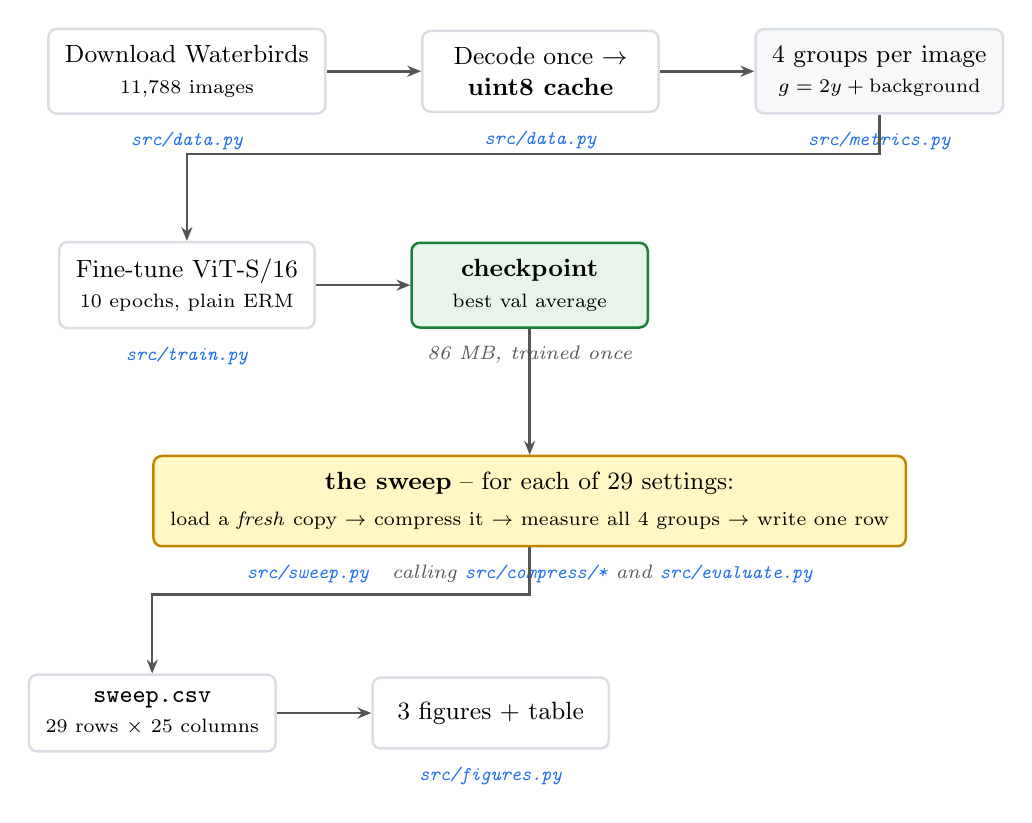
\begin{tikzpicture}[node distance=6mm]

% row 1: data prep
\node[blk,minimum width=30mm] (dl) {Download Waterbirds\\\scriptsize 11{,}788 images};
\node[blk,minimum width=30mm,right=12mm of dl] (cache) {Decode once $\to$\\\textbf{uint8 cache}};
\node[blkf,minimum width=30mm,right=12mm of cache] (split) {4 groups per image\\\scriptsize $g = 2y + \text{background}$};
\draw[ar] (dl)--(cache); \draw[ar] (cache)--(split);
\node[lbl,below=1mm of dl] {\f{src/data.py}};
\node[lbl,below=1mm of cache] {\f{src/data.py}};
\node[lbl,below=1mm of split] {\f{src/metrics.py}};

% row 2: training
\node[blk,minimum width=30mm,below=16mm of dl] (tr) {Fine-tune ViT-S/16\\\scriptsize 10 epochs, plain ERM};
\node[blkg,minimum width=30mm,right=12mm of tr] (ck) {\textbf{checkpoint}\\\scriptsize best val average};
\draw[ar] (split.south) -- ++(0,-5mm) -| (tr.north);
\draw[ar] (tr)--(ck);
\node[lbl,below=1mm of tr] {\f{src/train.py}};
\node[lbl,below=1mm of ck] {\scriptsize\itshape 86 MB, trained once};

% row 3: the sweep
\node[blkw,minimum width=74mm,below=16mm of ck,align=center] (sweep)
  {\textbf{the sweep} -- for each of 29 settings:\\[2pt]
   \scriptsize load a \emph{fresh} copy $\to$ compress it $\to$ measure all 4 groups $\to$ write one row};
\draw[ar] (ck.south) -- ++(0,-5mm) -| (sweep.north);
\node[lbl,below=1mm of sweep] {\f{src/sweep.py} \; calling \f{src/compress/*} and \f{src/evaluate.py}};

% row 4: outputs
\node[blk,minimum width=30mm,below=16mm of sweep.south west,anchor=north] (csv) {\code{sweep.csv}\\\scriptsize 29 rows $\times$ 25 columns};
\node[blk,minimum width=30mm,right=12mm of csv] (figs) {3 figures + table};
\draw[ar] (sweep.south) -- ++(0,-6mm) -| (csv.north);
\draw[ar] (csv)--(figs);
\node[lbl,below=1mm of figs] {\f{src/figures.py}};

\end{tikzpicture}
\end{center}

\noindent Read that top to bottom and you've got the shape of the repo. Now the
important bit about \emph{where} in the model the compression actually happens.

\subsection{What a ViT block looks like, and where we cut}

Our model is ViT-S/16: 12 identical blocks stacked on top of each other. Each
block has two halves -- an attention part and a feed-forward (MLP) part. Here's
one block, with the four weight matrices we're allowed to touch highlighted:

\begin{center}
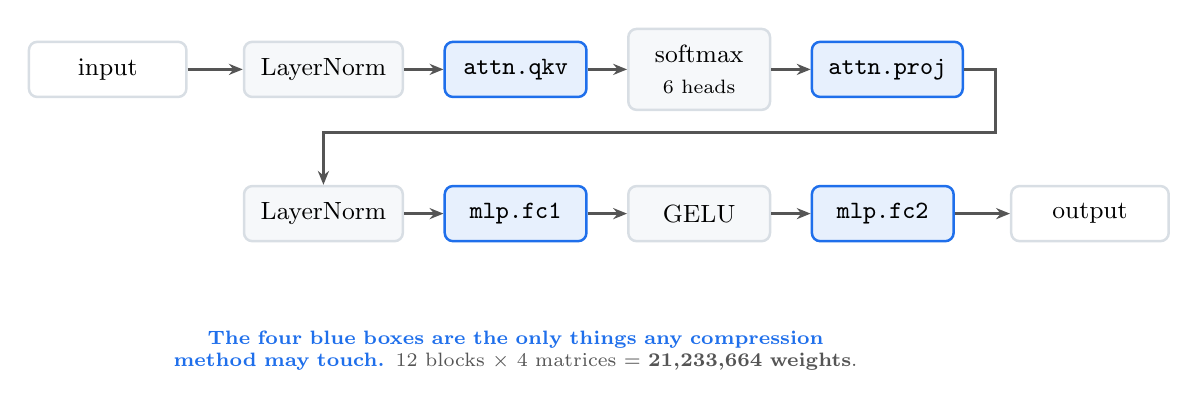
\begin{tikzpicture}[node distance=5mm]
\node[blk,minimum width=20mm,minimum height=7mm] (in) at (0,0) {input};

\node[blkf,minimum width=16mm,minimum height=7mm,right=7mm of in] (ln1) {LayerNorm};
\node[blka,minimum width=18mm,minimum height=7mm,right=5mm of ln1] (qkv) {\code{attn.qkv}};
\node[blkf,minimum width=18mm,minimum height=7mm,right=5mm of qkv] (sm) {softmax\\\scriptsize 6 heads};
\node[blka,minimum width=18mm,minimum height=7mm,right=5mm of sm] (proj) {\code{attn.proj}};

\draw[ar] (in)--(ln1); \draw[ar] (ln1)--(qkv); \draw[ar] (qkv)--(sm); \draw[ar] (sm)--(proj);

\node[blkf,minimum width=16mm,minimum height=7mm,below=11mm of ln1] (ln2) {LayerNorm};
\node[blka,minimum width=18mm,minimum height=7mm,right=5mm of ln2] (fc1) {\code{mlp.fc1}};
\node[blkf,minimum width=18mm,minimum height=7mm,right=5mm of fc1] (gelu) {GELU};
\node[blka,minimum width=18mm,minimum height=7mm,right=5mm of gelu] (fc2) {\code{mlp.fc2}};
\node[blk,minimum width=20mm,minimum height=7mm,right=7mm of fc2] (out) {output};

\draw[ar] (proj.east) -- ++(4mm,0) -- ++(0,-8mm) -| (ln2.north);
\draw[ar] (ln2)--(fc1); \draw[ar] (fc1)--(gelu); \draw[ar] (gelu)--(fc2); \draw[ar] (fc2)--(out);

\node[tiny,below=10mm of fc1,text width=95mm,align=center]
  {\textcolor{accent}{\bfseries The four blue boxes are the only things any compression
   method may touch.} 12 blocks $\times$ 4 matrices $=$ \textbf{21{,}233{,}664 weights}.};
\end{tikzpicture}
\end{center}

\begin{note}{accent}{The ``scope'' and why it's frozen}
Everything else -- the patch embedding, the position embeddings, the class
token, every LayerNorm, every bias, and the final classifier head -- is
\textbf{off limits}, for every method, always. That's the list in
\f{model.py} called \code{TARGET\_SUFFIXES}.

Why bother? Because ``we pruned 30\%'' has to mean the same thing in all four
experiments. If head removal were allowed to touch LayerNorms and magnitude
pruning wasn't, the sparsity numbers wouldn't be comparable and the whole
results table would be meaningless. One scope, decided once, reused everywhere.
\end{note}

\noindent And here's where each method attacks that scope:

\begin{center}
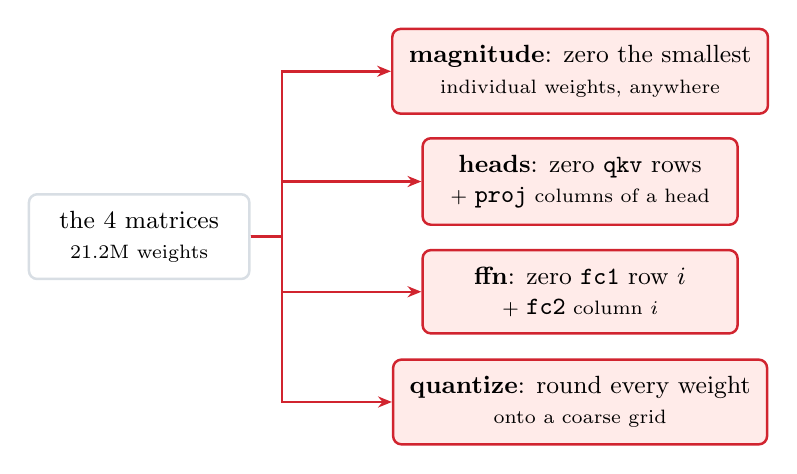
\begin{tikzpicture}[node distance=4mm]
\node[blk,minimum width=28mm,minimum height=8mm] (s) at (0,0) {the 4 matrices\\\scriptsize 21.2M weights};
\node[blkb,minimum width=40mm,minimum height=8mm] (m) at (5.6,2.1) {\textbf{magnitude}: zero the smallest\\\scriptsize individual weights, anywhere};
\node[blkb,minimum width=40mm,minimum height=8mm] (h) at (5.6,0.7) {\textbf{heads}: zero \code{qkv} rows\\\scriptsize $+$ \code{proj} columns of a head};
\node[blkb,minimum width=40mm,minimum height=8mm] (f) at (5.6,-0.7) {\textbf{ffn}: zero \code{fc1} row $i$\\\scriptsize $+$ \code{fc2} column $i$};
\node[blkb,minimum width=40mm,minimum height=8mm] (q) at (5.6,-2.1) {\textbf{quantize}: round every weight\\\scriptsize onto a coarse grid};
\foreach \n in {m,h,f,q} {\draw[arb] (s.east) -- ++(4mm,0) |- (\n.west);}
\end{tikzpicture}
\end{center}


% ================================================================ PART 3
\section{Every file, one by one}

Read them in this order -- each one only depends on the ones above it.

\begin{center}
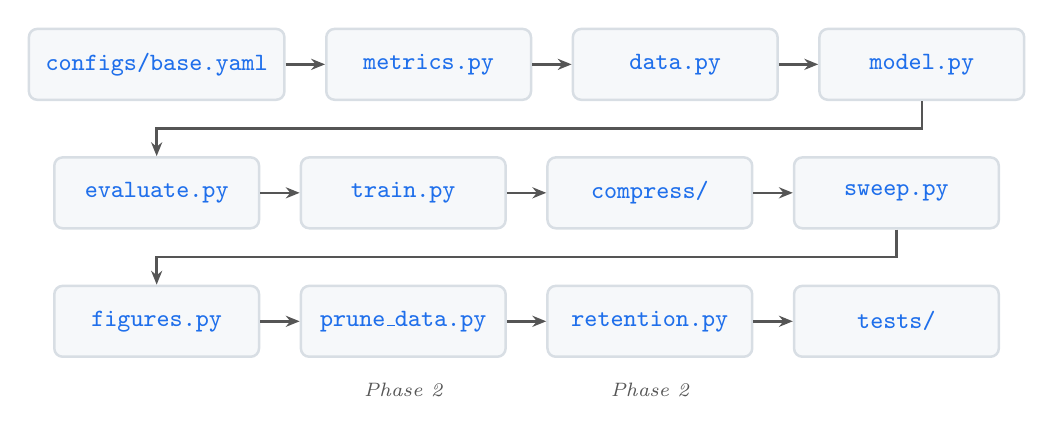
\begin{tikzpicture}[node distance=3mm]
\node[blkf,minimum width=26mm] (c) {\f{configs/base.yaml}};
\node[blkf,minimum width=26mm,right=5mm of c] (me) {\f{metrics.py}};
\node[blkf,minimum width=26mm,right=5mm of me] (da) {\f{data.py}};
\node[blkf,minimum width=26mm,right=5mm of da] (mo) {\f{model.py}};
\draw[ar] (c)--(me); \draw[ar] (me)--(da); \draw[ar] (da)--(mo);

\node[blkf,minimum width=26mm,below=7mm of c] (ev) {\f{evaluate.py}};
\node[blkf,minimum width=26mm,right=5mm of ev] (trn) {\f{train.py}};
\node[blkf,minimum width=26mm,right=5mm of trn] (cp) {\f{compress/}};
\node[blkf,minimum width=26mm,right=5mm of cp] (sw) {\f{sweep.py}};
\draw[ar] (mo.south) -- ++(0,-3.5mm) -| (ev.north);
\draw[ar] (ev)--(trn); \draw[ar] (trn)--(cp); \draw[ar] (cp)--(sw);

\node[blkf,minimum width=26mm,below=7mm of ev] (fg) {\f{figures.py}};
\node[blkf,minimum width=26mm,right=5mm of fg] (pd) {\f{prune\_data.py}};
\node[blkf,minimum width=26mm,right=5mm of pd] (rt) {\f{retention.py}};
\node[blkf,minimum width=26mm,right=5mm of rt] (ts) {\f{tests/}};
\draw[ar] (sw.south) -- ++(0,-3.5mm) -| (fg.north);
\draw[ar] (fg)--(pd); \draw[ar] (pd)--(rt); \draw[ar] (rt)--(ts);
\node[lbl,below=2mm of pd] {Phase 2};
\node[lbl,below=2mm of rt] {Phase 2};
\end{tikzpicture}
\end{center}

\subsection{\texttt{configs/base.yaml} -- every number lives here}

\textbf{What it does:} holds every constant the pipeline depends on. Learning
rate, epochs, which sparsity levels to sweep, where files go.

\textbf{Why it exists:} so no number is hardcoded in two places. If you want to
sweep different sparsity levels, you edit this file and nothing else.

\textbf{Look at:} the \code{sweep:} block -- those lists are literally the 29
experiments. \code{magnitude\_sparsity} has 7 values, \code{heads\_removed} 7,
\code{ffn\_fraction} 7, and quantize is 4 bit-widths $\times$ 2 granularities
$=$ 8. That's $7+7+7+8 = 29$.

\subsection{\texttt{src/metrics.py} -- what ``group'' and ``worst group'' mean}

\textbf{What it does:} turns predictions into group-aware accuracy numbers. No
model code, no PyTorch layers -- just counting.

\textbf{The one function to understand:}

\begin{center}
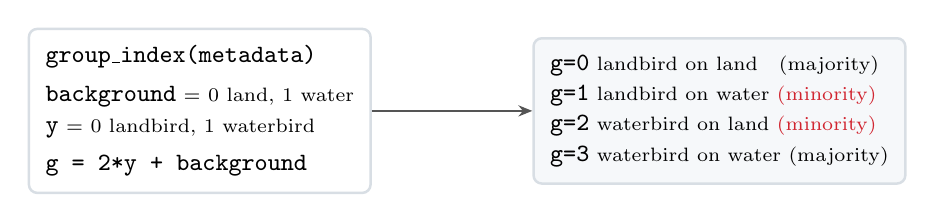
\begin{tikzpicture}
\node[blk,minimum width=42mm,align=left] (a) at (0,0)
  {\code{group\_index(metadata)}\\[3pt]
   \scriptsize \code{background} $=$ 0 land, 1 water\\
   \scriptsize \code{y} $=$ 0 landbird, 1 waterbird\\[3pt]
   \code{\textbf{g = 2*y + background}}};
\node[blkf,minimum width=46mm,align=left] (b) at (6.6,0)
  {\scriptsize \code{g=0} landbird on land \; (majority)\\
   \scriptsize \code{g=1} landbird on water \textcolor{bad}{(minority)}\\
   \scriptsize \code{g=2} waterbird on land \textcolor{bad}{(minority)}\\
   \scriptsize \code{g=3} waterbird on water (majority)};
\draw[ar] (a)--(b);
\end{tikzpicture}
\end{center}

\textbf{The tricky bit:} \code{adjusted\_average}. It does \emph{not} compute a
plain mean. It takes per-group accuracy and reweights by how common each group
was \textbf{in training} (72.9\%, 3.8\%, 1.2\%, 22.0\%). That's why our headline
is 98.2\% and not 91.7\%. Both are correct; they answer different questions.

\textbf{Also note:} \code{TRAIN\_GROUP\_COUNTS = [3498, 184, 56, 1057]} is
asserted against the real data by a test. If that assert ever fails, group
indexing is wrong and every number downstream is garbage. It's a tripwire.

\subsection{\texttt{src/data.py} -- loading images, fast}

\textbf{What it does:} downloads Waterbirds, reads \code{metadata.csv}, exposes
the three official splits, and builds the uint8 caches.

\textbf{Why the cache exists:} we evaluate the test set about 30 times during a
sweep. Decoding 5{,}794 JPEGs each time would dominate everything. So we decode
once, resize once, and keep raw pixels in a big tensor.

\begin{center}
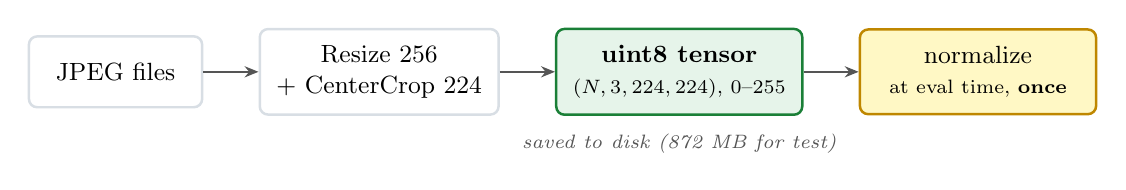
\begin{tikzpicture}[node distance=5mm]
\node[blk,minimum width=22mm] (j) {JPEG files};
\node[blk,minimum width=28mm,right=7mm of j] (r) {Resize 256\\$+$ CenterCrop 224};
\node[blkg,minimum width=30mm,right=7mm of r] (u) {\textbf{uint8 tensor}\\\scriptsize $(N,3,224,224)$, 0--255};
\node[blkw,minimum width=30mm,right=7mm of u] (n) {normalize\\\scriptsize at eval time, \textbf{once}};
\draw[ar] (j)--(r); \draw[ar] (r)--(u); \draw[ar] (u)--(n);
\node[lbl,below=1mm of u] {saved to disk (872 MB for test)};
\end{tikzpicture}
\end{center}

\begin{note}{bad}{The double-normalize trap}
Notice the cache stores \textbf{raw 0--255 pixels}, not normalized floats. That's
deliberate and it's the single easiest way to wreck this project.

If you normalized before caching, and then the eval code normalized again (which
it does, every time), every image would be silently wrong. Your accuracy would
drop a bit, nothing would crash, and you'd spend a week blaming compression. The
comment in the file calls this ``the double-normalize trap''. Caching
pre-normalization is what avoids it.
\end{note}

\textbf{Look at:} \code{normalize\_uint8()} -- it's three lines and it's the only
place normalization ever happens.

\subsection{\texttt{src/model.py} -- building the model and freezing the scope}

\textbf{What it does:} creates the ViT, loads checkpoints, and defines exactly
which weights compression may touch.

\textbf{Two functions that matter:}

\begin{itemize}[leftmargin=1.4em]
\item \code{targeted\_named\_weights(model)} -- returns the list of
\textbf{21{,}233{,}664} weights in scope. Every compression method starts by
calling this. One definition, four methods.

\item \code{fresh\_model(ckpt, device)} -- loads a brand new, clean, untouched
model from the checkpoint file. The sweep calls this so that every configuration
starts from the same pristine weights.
\end{itemize}

\textbf{Also:} \code{assert\_structure()} checks the model really is
12 blocks $\times$ 6 heads $\times$ 64 dims, that \code{attn.norm} is an
\code{Identity}, and that the matrices have the shapes we expect. This isn't
paranoia -- the head-removal maths in Section~\ref{sec:tricky} is only correct \emph{because} of
that layout. If a future version of \code{timm} changes it, this assert fires
instead of silently producing wrong results.

\subsection{\texttt{src/evaluate.py} -- one measurement pass}

\textbf{What it does:} runs the model over a cached split and returns the full
metric dict. It's 50 lines and you can read it in a minute.

\textbf{The one line to notice:} \code{model.eval()} at the top. Without it,
dropout and drop-path stay active and inject random noise -- which would look
exactly like a compression effect. The comment says so.

\textbf{Also returns \code{pred\_mean}}, the average predicted class. This is the
collapse detector; see Section~\ref{sec:tricky}.

\subsection{\texttt{src/train.py} -- fine-tuning, deliberately naive}

\textbf{What it does:} takes a model pretrained on ImageNet, swaps in a 2-class
head, and fine-tunes on Waterbirds for 10 epochs. AdamW, learning rate 1e-5,
cosine schedule, batch size 32.

\textbf{What it deliberately does NOT do:} no group labels, no reweighted loss,
no balanced sampler, no GroupDRO, nothing clever. Plain shuffling, plain
cross-entropy.

\begin{note}{warn}{``Why would you train it badly on purpose?''}
Because the model is \emph{supposed} to learn the shortcut. That's the thing we
want to study. If we trained it group-balanced, worst-group accuracy would start
around 90\%, there'd be no gap, and compression would have nothing interesting
to break. The naive model is the subject of the experiment, not a mistake.
\end{note}

\textbf{The subtle choice -- which epoch do we keep?} We save the checkpoint
with the best \textbf{plain validation average} accuracy. Not worst-group. Here's
why that matters:

\begin{center}
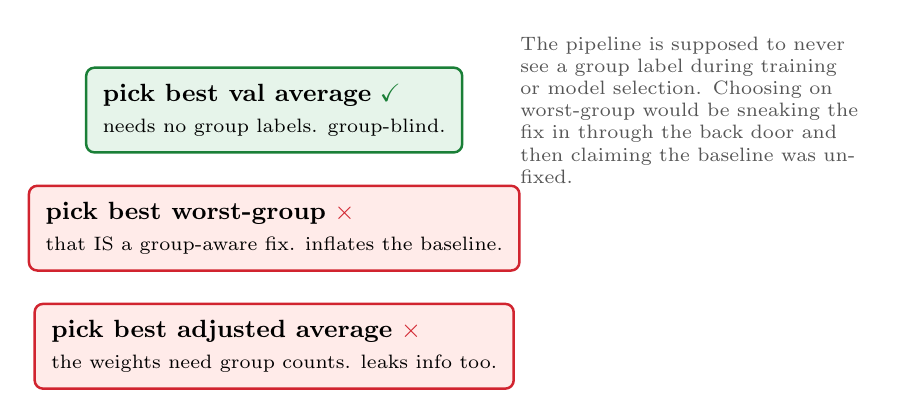
\begin{tikzpicture}[node distance=4mm]
\node[blkg,minimum width=44mm,minimum height=10mm,align=left] (ok) at (0,0)
  {\textbf{pick best val average} \textcolor{good}{\checkmark}\\\scriptsize needs no group labels. group-blind.};
\node[blkb,minimum width=44mm,minimum height=10mm,align=left] (no1) at (0,-1.5)
  {\textbf{pick best worst-group} \textcolor{bad}{$\times$}\\\scriptsize that IS a group-aware fix. inflates the baseline.};
\node[blkb,minimum width=44mm,minimum height=10mm,align=left] (no2) at (0,-3.0)
  {\textbf{pick best adjusted average} \textcolor{bad}{$\times$}\\\scriptsize the weights need group counts. leaks info too.};
\node[tiny,right=6mm of ok,text width=44mm,align=left]
  {The pipeline is supposed to never see a group label during training or model
   selection. Choosing on worst-group would be sneaking the fix in through the
   back door and then claiming the baseline was unfixed.};
\end{tikzpicture}
\end{center}

\textbf{What Phase 2 added to this file}: \code{prune\_indices} to train on a
subset, \code{score\_epoch} to record per-sample difficulty, and
\code{stop\_after\_epoch} to score a model without overwriting an existing
checkpoint. Section~\ref{sec:phase2} explains what those are for.

Three more flags exist only because a long unattended run went wrong, and they
are worth knowing about if you ever leave this training overnight:

\begin{itemize}[leftmargin=1.4em]
\item \code{--resume} picks a killed run back up from where it stopped, putting
the optimiser and the learning-rate schedule back exactly as they were. Without
that last part you'd restart mid-schedule and get a model that looks fine and
isn't.
\item \code{--allow-overwrite} is a refusal, not a feature. A fresh run will not
start on top of a model that already exists unless you say this. Saved models
are not backed up anywhere and cost half an hour each to rebuild.
\item \code{--num-workers} loads images on several threads. It is set to 0,
which sounds wrong but was measured: it made no difference to speed here, and 0
reproduces Phase 1's results exactly, so 0 it is.
\end{itemize}

\begin{note}{bad}{The bug these came from}
\code{stop\_after\_epoch} exists to score a model \emph{without} touching the
saved copy. Its check was one line too late, so a scoring run reached the
``save if this is the best so far'' step first and overwrote the Phase 1 model
with a much worse, half-trained one. The flag whose only job was to protect that
file is what destroyed it.

Nothing noticed -- the replacement looked like a perfectly normal model. It had
to be retrained from scratch, which worked only because training here turns out
to be exactly repeatable: all ten epochs came back identical to the original.
Gate V13 now checks this specific case, and \f{preflight.py} re-checks every
saved model against the record of how it was trained before any long run starts.
\end{note}

\subsection{\texttt{src/compress/} -- the four methods, one contract}

Every method, without exception, follows the same shape:

\begin{center}

\begin{tikzpicture}
\node[blk,minimum width=100mm,align=center,font=\small]
  {\code{apply(model, **params) -> (new\_model, stats)}};
\end{tikzpicture}\\[4pt]
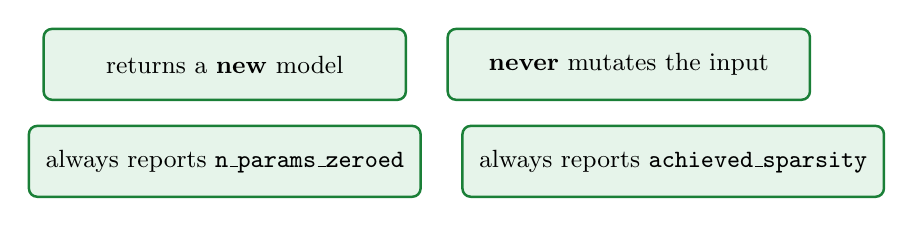
\begin{tikzpicture}[node distance=4mm]
\node[blkg,minimum width=46mm] (a) {returns a \textbf{new} model};
\node[blkg,minimum width=46mm,right=5mm of a] (b) {\textbf{never} mutates the input};
\node[blkg,minimum width=46mm,below=3mm of a] (c) {always reports \code{n\_params\_zeroed}};
\node[blkg,minimum width=46mm,right=5mm of c] (d) {always reports \code{achieved\_sparsity}};
\end{tikzpicture}
\end{center}

\noindent That contract is enforced by tests, not by good intentions. The shared
helper \code{clone\_model()} in \code{\_common.py} is a deep copy -- that's where
``never mutates'' starts.

\begin{note}{accent}{Masking, not shrinking}
Two of the methods (heads, ffn) delete whole structural chunks. You might expect
them to physically make the tensors smaller. They don't -- they set things to
zero and leave the shapes alone.

Why: so \code{achieved\_sparsity} means the same thing for all four methods. If
head removal physically narrowed \code{qkv}, then ``fraction of targeted weights
zeroed'' would be measuring something different than it does under magnitude
pruning, and you couldn't put them on the same axis. The tests prove the masked
version gives \emph{bit-identical} outputs to really deleting the parts.
\end{note}

\subsubsection*{\texttt{magnitude.py} -- zero the smallest weights}

Take all 21.2M weights, sort by absolute value, zero the smallest $k$ of them.
Global ranking: a tiny weight in block 11 gets pruned before a big weight in
block 0.

\begin{center}
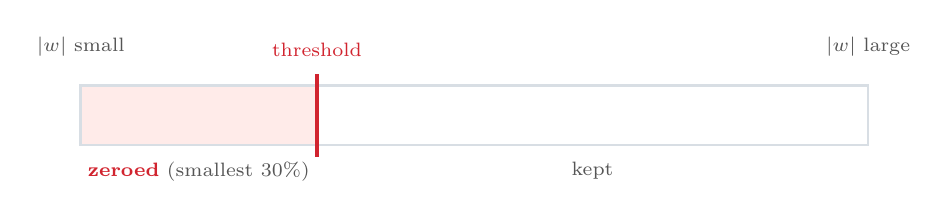
\begin{tikzpicture}
\draw[draw=rule,line width=0.9pt] (0,0) rectangle (10,0.75);
\fill[badbg] (0,0) rectangle (3,0.75);
\draw[draw=rule,line width=0.9pt] (0,0) rectangle (10,0.75);
\draw[bad,line width=1.3pt] (3,-0.15) -- (3,0.9);
\node[tiny,below=1mm of {(1.5,0)}] {\textcolor{bad}{\bfseries zeroed} (smallest 30\%)};
\node[tiny,below=1mm of {(6.5,0)}] {kept};
\node[tiny,above=1mm of {(3,0.9)},bad] {threshold};
\node[tiny,above=1mm of {(0,0.9)}] {$|w|$ small};
\node[tiny,above=1mm of {(10,0.9)}] {$|w|$ large};
\end{tikzpicture}
\end{center}

\textbf{The tricky bit -- ties.} With 21 million float32 numbers, the threshold
value is \emph{not unique}. Several weights have exactly the same magnitude
(measured: ties run 1--3 deep). If you wrote the obvious mask
\code{w.abs() > threshold}, you'd zero \emph{every} tied weight and overshoot
your target. You'd ask for 30\% and get 30.0001\%.

So the code zeroes everything strictly below the threshold, counts how many that
was, and then spends an explicit ``tie budget'' on exactly as many tied weights
as it still needs -- in a fixed order so it's reproducible. Result: exactly $k$
weights, every time. That's why the test is an equality and not a
``close enough''.

\subsubsection*{\texttt{heads.py} -- delete whole attention heads}

Each block has 6 attention heads. A head owns a specific slice of two matrices:

\begin{center}
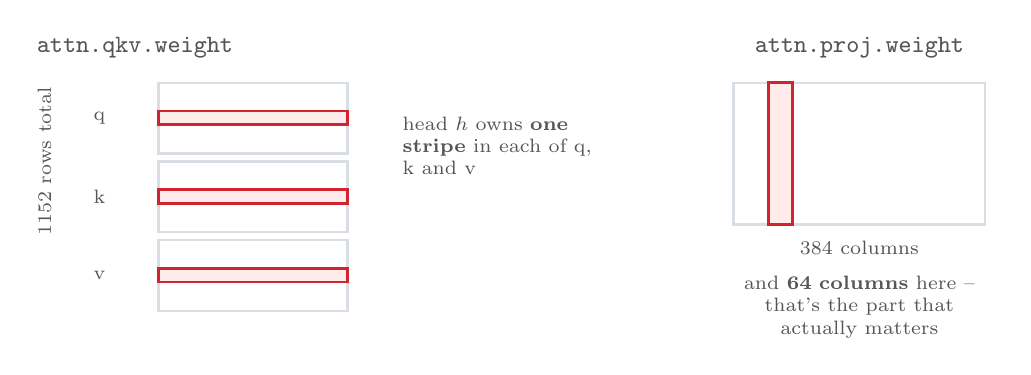
\begin{tikzpicture}
% qkv
\node[tiny] at (-0.3,3.55) {\code{attn.qkv.weight}};
\node[tiny,rotate=90] at (-1.45,2.1) {1152 rows total};
\foreach \i/\lab in {0/q,1/k,2/v} {
  \draw[draw=rule,line width=0.8pt] (0,3.1-\i*1.0) rectangle (2.4,2.2-\i*1.0);
  \node[tiny] at (-0.75,2.65-\i*1.0) {\lab};
  \fill[badbg,draw=bad,line width=1pt] (0,2.74-\i*1.0) rectangle (2.4,2.57-\i*1.0);
}
\node[tiny,text width=26mm,align=left] at (4.4,2.3)
  {head $h$ owns \textbf{one stripe} in each of q, k and v};

% proj
\node[tiny] at (8.9,3.55) {\code{attn.proj.weight}};
\draw[draw=rule,line width=0.8pt] (7.3,3.1) rectangle (10.5,1.3);
\fill[badbg,draw=bad,line width=1pt] (7.75,3.1) rectangle (8.05,1.3);
\node[tiny] at (8.9,1.0) {384 columns};
\node[tiny,text width=34mm,align=center] at (8.9,0.25)
  {and \textbf{64 columns} here --\\that's the part that actually matters};
\end{tikzpicture}
\end{center}

\textbf{Why zeroing those columns genuinely deletes the head.} At the end of
attention, the 6 heads' outputs are laid side by side into one long vector, and
then \code{proj} maps it back down. Head $h$'s output lands in columns
$[h \cdot 64, (h{+}1)\cdot 64)$ of that vector. Zero those columns of
\code{proj} and head $h$ contributes \textbf{exactly nothing} to the output.
Not approximately -- exactly.

The \code{qkv} rows get zeroed too. They can't change the output anymore (proj
already blocks it), but they \emph{are} dead weight, and leaving them out of the
count would understate how much of the model a head sweep removes.

\textbf{One guard rail:} at least 1 head must survive per block. Empty a block's
attention completely and it stops being a compressed transformer and becomes a
different architecture -- and the accuracy cliff would get blamed on ``head
sparsity''. 12 blocks $\times$ 5 removable $=$ 60 max, which is exactly where
the sweep stops.

\subsubsection*{\texttt{ffn.py} -- delete whole MLP neurons}

Simplest one conceptually. A ``neuron'' in the feed-forward layer is a matched
pair: row $i$ of \code{fc1} (which computes it) and column $i$ of \code{fc2}
(the only way it reaches the output).

\begin{center}
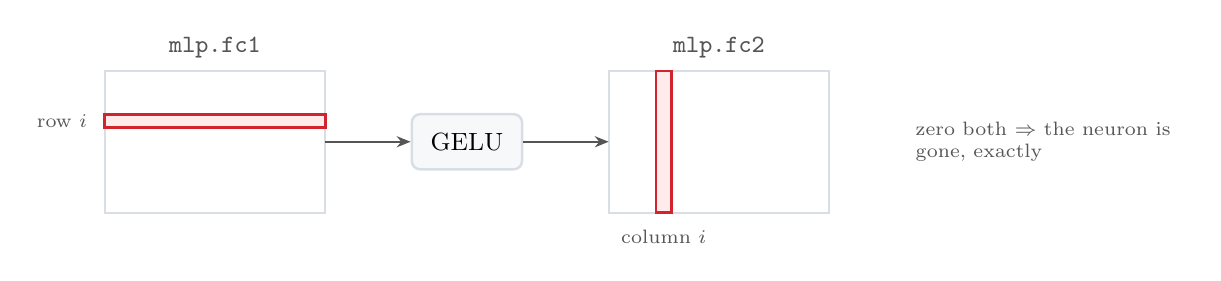
\begin{tikzpicture}
\node[tiny] at (1.4,2.3) {\code{mlp.fc1}};
\draw[draw=rule,line width=0.8pt] (0,2.0) rectangle (2.8,0.2);
\fill[badbg,draw=bad,line width=1pt] (0,1.45) rectangle (2.8,1.28);
\node[tiny,left=1mm of {(0,1.36)}] {row $i$};

\node[blkf,minimum width=14mm,minimum height=7mm] (g) at (4.6,1.1) {GELU};
\draw[ar] (2.8,1.1)--(g.west);

\node[tiny] at (7.8,2.3) {\code{mlp.fc2}};
\draw[draw=rule,line width=0.8pt] (6.4,2.0) rectangle (9.2,0.2);
\fill[badbg,draw=bad,line width=1pt] (7.0,2.0) rectangle (7.2,0.2);
\draw[ar] (g.east)--(6.4,1.1);
\node[tiny,below=1mm of {(7.1,0.2)}] {column $i$};

\node[tiny,text width=34mm,align=left] at (12.0,1.1)
  {zero both $\Rightarrow$ the neuron is gone, exactly};
\end{tikzpicture}
\end{center}

\textbf{The ``wait, what about the bias?'' question.} \code{fc1.bias} is
\emph{not} zeroed -- biases are outside the frozen scope. So a pruned neuron
still outputs a constant \code{GELU(bias\_i)}. Doesn't that break exactness?

No. That constant gets multiplied by \code{fc2}'s zeroed column, so it
contributes exactly zero. Removal stays exact without widening the scope. Nice
little result, and there's a test that checks it against a reference model.

\textbf{No per-block floor here}, unlike heads. Emptying one block's MLP leaves
attention and the residual stream intact -- it degrades the model rather than
changing its architecture. So blocks are free to give up wildly different
numbers of neurons, and where the ranking chooses to cut is itself a result.

\subsubsection*{\texttt{quantize.py} -- fewer bits per weight}

Instead of removing weights, store each one with less precision. Round every
weight onto an evenly spaced grid.

\begin{center}
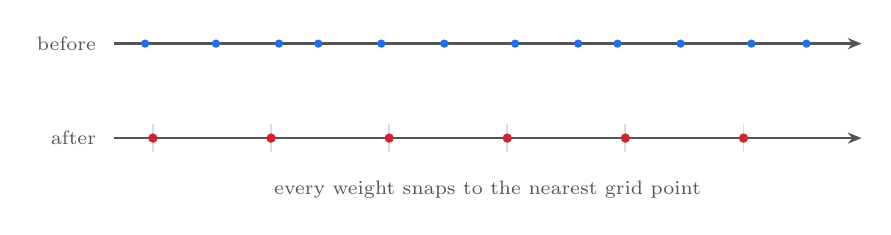
\begin{tikzpicture}
\draw[ar,draw=ink2] (0,1.2)--(9.5,1.2);
\foreach \x in {0.4,1.3,2.1,2.6,3.4,4.2,5.1,5.9,6.4,7.2,8.1,8.8}
  {\fill[accent] (\x,1.2) circle (1.5pt);}
\node[tiny,left=1mm of {(0,1.2)}] {before};

\draw[ar,draw=ink2] (0,0)--(9.5,0);
\foreach \x in {0.5,2.0,3.5,5.0,6.5,8.0} {\draw[rule,line width=0.7pt] (\x,-0.18)--(\x,0.18);}
\foreach \x/\n in {0.5/2,2.0/2,3.5/2,5.0/2,6.5/2,8.0/2} {\fill[bad] (\x,0) circle (1.7pt);}
\node[tiny,left=1mm of {(0,0)}] {after};
\node[tiny] at (4.75,-0.65) {every weight snaps to the nearest grid point};
\end{tikzpicture}
\end{center}

\textbf{Two knobs, and one matters more than you'd think:}

\begin{itemize}[leftmargin=1.4em]
\item \textbf{bits} -- 8, 6, 4, or 3. Fewer bits $=$ coarser grid.
\item \textbf{granularity} -- \code{per\_tensor} uses one grid spacing for the
whole matrix; \code{per\_channel} uses a separate one for each output row.
\end{itemize}

\noindent At 4 bits, per-channel keeps \textbf{60.6\%} worst-group accuracy and
per-tensor keeps \textbf{23.8\%}. Same bit budget, wildly different outcome. One
big outlier weight ruins the grid spacing for the entire tensor, and per-channel
contains the damage to one row.

\textbf{Note:} this is \emph{simulated} quantization -- quantize then dequantize
back to float32. We're measuring accuracy, not speed, and the numerical effect is
reproduced exactly. Real int4 kernels are CUDA-only and wouldn't change a single
accuracy number.

\textbf{Tiny detail worth knowing:} at \code{bits=32} the code short-circuits and
returns the model untouched. If it actually ran the maths, dividing by a scale
that small would push values past what float32's mantissa can hold, and the
``identity'' would be off by about 1e-7 -- failing a test that demands exact
identity.

\subsection{\texttt{src/sweep.py} -- the thing that actually runs the experiment}

\textbf{What it does:} loops over all 29 configurations. For each one: load a
fresh model, compress it, evaluate it, write a row to \code{results/sweep.csv}.

This is the most important file in the repo and it exists mostly to protect two
invariants.

\begin{center}
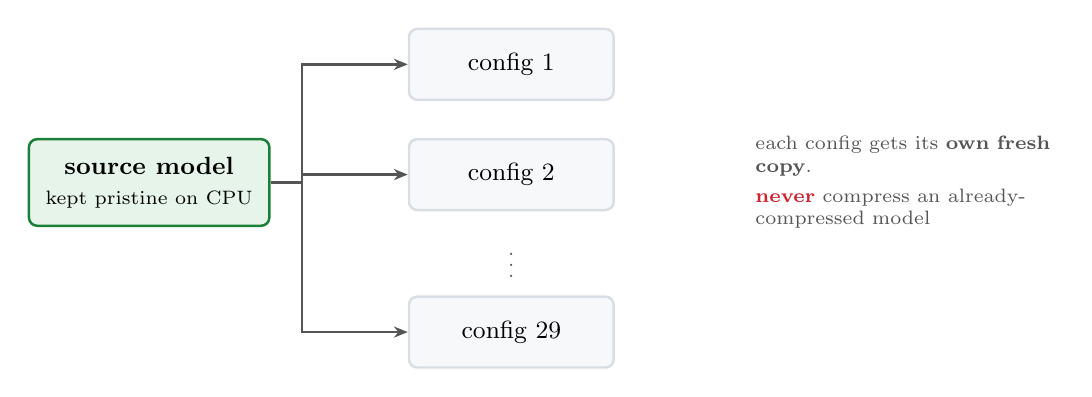
\begin{tikzpicture}[node distance=5mm]
\node[blkg,minimum width=30mm,minimum height=11mm] (src) at (0,0)
  {\textbf{source model}\\\scriptsize kept pristine on CPU};
\node[blkf,minimum width=26mm,minimum height=9mm] (c1) at (4.6,1.5) {config 1};
\node[blkf,minimum width=26mm,minimum height=9mm] (c2) at (4.6,0.1) {config 2};
\node[tiny] at (4.6,-0.95) {\vdots};
\node[blkf,minimum width=26mm,minimum height=9mm] (c3) at (4.6,-1.9) {config 29};
\foreach \n in {c1,c2,c3} {\draw[ar] (src.east) -- ++(4mm,0) |- (\n.west);}
\node[tiny,text width=38mm,align=left] at (9.6,0)
  {each config gets its \textbf{own fresh copy}.\\[3pt]
   \textcolor{bad}{\bfseries never} compress an already-compressed model};
\end{tikzpicture}
\end{center}

\begin{note}{bad}{The most dangerous bug available in this project}
If config 2 accidentally compressed the output of config 1, the damage would
compound. And here's the evil part: \textbf{the output would still look
completely plausible.} You'd get smooth, believable curves that are entirely
wrong, and nothing would crash or look weird.

So the code doesn't just trust the control flow. Before every single config it
recomputes a \code{\_fingerprint()} of the source model -- the count of zeros
plus the sum of all weights -- and asserts it hasn't changed. If any compression
method ever broke its ``don't mutate the input'' promise, that assert fires
immediately instead of 29 rows later.
\end{note}

\textbf{Invariant 2: resumability.} Each row is written and flushed to disk the
moment it's done. A sweep is $\sim$30 full passes over 5{,}794 images; if your
laptop sleeps halfway through, \code{--resume} picks up from the last finished
row instead of starting over.

\textbf{Look at:} \code{run\_one()} -- it's about 25 lines and it's the entire
experiment in miniature: compress, evaluate, build a row.

\subsection{\texttt{src/figures.py} -- turning the CSV into pictures}

\textbf{What it does:} reads \code{sweep.csv} plus \code{baseline.json} and
writes the three figures and the summary table.

\textbf{The one concept:} collapsed configurations are drawn as \emph{hollow}
markers and excluded from the trade-off plot. Section~\ref{sec:tricky} explains why that matters
so much.

\subsection{Phase 2 files}

\textbf{\f{src/prune\_data.py}} -- scores every training image by how ``hard'' it
is, then removes the hardest ones and writes a list of which images to keep. It
holds \emph{two} rules, chosen with \code{--variant}: \code{global} deletes the
hardest images anywhere (the version that failed), and \code{spurious} deletes
only from the groups where the background agrees with the bird (the version that
works). See Section~\ref{sec:phase2}.

\textbf{\f{src/retention.py}} -- compares the ERM model against the pruned model
at matched compression and computes the retention ratio. This is Phase 2's
headline number.

\textbf{\f{src/migrate\_csv.py}} -- a one-shot utility that adds the new
\code{tag} column to the Phase 1 CSV so both phases share one schema. You'll
never run it again.

\textbf{\f{run\_phase2.sh}} -- runs the whole Phase 2 pipeline in stages. Every
step skips if its output already exists, so an interrupted night resumes by just
running it again. Two stages exist only because an overnight run went wrong
once: \textbf{stage 0} checks everything up front -- disk space, the image
caches, and whether each saved model still matches the record of how it was
trained -- and refuses to start if anything is off. \textbf{Stage 5} checks
afterwards whether every piece of work really finished, by looking at the files
rather than the log.

\textbf{\f{src/preflight.py}} and \textbf{\f{src/verify.py}} are those two
checks. \f{verify.py} is the one to run if you ever want a straight answer to
``did it all actually finish?'' -- it reads the output files and says yes or no.
The log is not a reliable guide: on one run, 12 steps reported failure and 11 of
them had in fact completed their work and only tripped on the way out, when the
disk filled up.

\textbf{\f{src/progress.py}} -- prints the progress bar you can watch during a
long run.

\subsection{\texttt{tests/} -- the safety net}

64 tests, plus 15 more that drive the run script itself. They're not there for
code coverage points; each one pins down a
specific claim the rest of the code makes. The source comments literally refer
to them by number (``V4 is an equality check'').

\begin{center}
\begin{tabular}{@{}lll@{}}
\toprule
\textbf{Gate} & \textbf{Claims} & \textbf{Why you'd care} \\
\midrule
V1  & group counts are \code{[3498,184,56,1057]} & group indexing is right \\
V3  & quantize at 32 bits is identity & the method has no hidden bias \\
V4  & magnitude zeroes \emph{exactly} $k$ & the tie handling works \\
V5  & masking $=$ real deletion, bit for bit & structured removal is exact \\
V7b & the baseline hasn't collapsed & accuracy isn't a mirage \\
V8  & \code{apply} never mutates its input & the sweep is trustworthy \\
V10 & pruned set is class-balanced & Phase 2 removal is fair \\
V12 & resume key separates seeds & a 2nd seed doesn't silently skip \\
V13 & a cut-short run saves no model & it once destroyed the Phase 1 model \\
V14 & Python and the shell agree on a name & else half-trained models look done \\
V15 & the run script's skip/resume logic & an interrupted night resumes right \\
V17 & the fix never deletes a weak-group image & the whole point of the fix \\
V18 & the fix evens up the two classes & matches what the paper describes \\
\bottomrule
\end{tabular}
\end{center}

\noindent Run them with \code{pytest tests/ -q}. Takes about 35 seconds.

\begin{note}{warn}{Why there are suddenly more of these}
V13--V18 all exist because something went wrong on a real overnight run. V13 is
the sharpest: the flag whose entire job was to stop the Phase 1 model being
overwritten had its guard in the wrong place, and overwrote it. The model had to
be retrained from scratch to get it back. Each of those gates is one specific
mistake that can no longer repeat silently.
\end{note}


% ================================================================ PART 4
\section{How to read the figures}\label{sec:figures}

Running \f{figures.py} gives you three pictures and one table per model. They
all follow the same handful of rules, so once you can read one you can read all
of them. This section is those rules.

\begin{note}{accent}{The single most important convention}
A \textbf{filled dot} is a real measurement. A \textbf{hollow dot} is a model
that has stopped working -- it has given up and started answering almost every
image the same way. Hollow dots are drawn so the line still connects, but
\textbf{you must not read anything into them}. Section~\ref{sec:tricky}
explains why a broken model can look like it has a small gap.
\end{note}

\subsection{Figure 1 -- average vs worst group}

Five small plots, one per compression method. In each one:

\begin{itemize}[leftmargin=1.4em]
\item \textbf{Left to right} always means \emph{more compression}. For the
quantization plots that means the number of bits \emph{decreases} left to right
(8, 6, 4, 3), because fewer bits is more squeezing. The axis is deliberately
flipped so that ``worse'' is always rightward in every panel.
\item \textbf{Up and down} is test accuracy, always on the same 0--100\% scale
so the five panels are directly comparable.
\item \textbf{Two lines.} The upper one is average accuracy -- what a normal
evaluation would report. The lower one is worst-group accuracy.
\end{itemize}

\textbf{What you are looking for: the vertical distance between the two lines,
and how fast it opens up.} That gap is the whole finding. If the two lines fell
together, compression would be fair. They don't.

\begin{center}
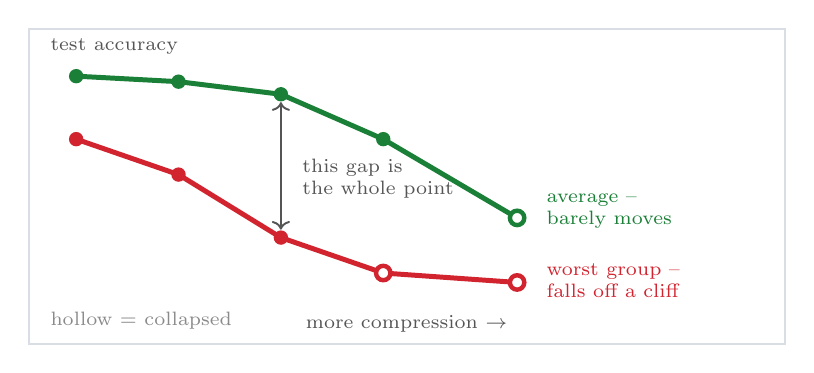
\begin{tikzpicture}[scale=1.0]
\draw[draw=rule,line width=0.9pt] (0,0) rectangle (9.6,4.0);
\node[tiny,anchor=west] at (0.15,3.78) {test accuracy};
\node[tiny,anchor=east] at (6.2,0.26) {more compression $\rightarrow$};
% average line: barely drops
\draw[good,line width=1.8pt] (0.6,3.40) -- (1.9,3.33) -- (3.2,3.17) -- (4.5,2.60) -- (6.2,1.60);
\foreach \x/\y in {0.6/3.40,1.9/3.33,3.2/3.17,4.5/2.60} \fill[good] (\x,\y) circle (2.6pt);
\fill[white] (6.2,1.60) circle (2.6pt); \draw[good,line width=1.6pt] (6.2,1.60) circle (2.6pt);
% worst group line: falls off
\draw[bad,line width=1.8pt] (0.6,2.60) -- (1.9,2.15) -- (3.2,1.35) -- (4.5,0.90) -- (6.2,0.78);
\foreach \x/\y in {0.6/2.60,1.9/2.15,3.2/1.35} \fill[bad] (\x,\y) circle (2.6pt);
\foreach \x/\y in {4.5/0.90,6.2/0.78} {\fill[white] (\x,\y) circle (2.6pt);
  \draw[bad,line width=1.6pt] (\x,\y) circle (2.6pt);}
% labels sit to the RIGHT of where each line ends, so nothing can overlap
\node[tiny,text=good,anchor=west,align=left] at (6.45,1.68) {average --\\barely moves};
\node[tiny,text=bad,anchor=west,align=left] at (6.45,0.80) {worst group --\\falls off a cliff};
\draw[<->,draw=ink2,line width=0.7pt] (3.2,1.45) -- (3.2,3.07);
\node[tiny,anchor=west,align=left] at (3.35,2.10) {this gap is\\the whole point};
\node[tiny,text=muted,anchor=west] at (0.15,0.30) {hollow = collapsed};
\end{tikzpicture}
\end{center}

\subsection{Figure 2 -- the same average, very different worst group}

One scatter plot. Each dot is one of the 29 compression settings. Left--right is
average accuracy, up--down is worst-group accuracy.

\textbf{How to read it: pick a spot on the horizontal axis and look up.} You
will find several dots stacked vertically. Those are compression settings that a
standard evaluation would call \emph{equally good} -- same average accuracy --
sitting at wildly different worst-group accuracies. That vertical spread is the
information the average throws away. The further a dot sits below the others at
its own horizontal position, the more that particular setting hurt the group
that was already weakest.

\subsection{Figure 3 -- which group actually pays}

Five panels again, same axes as Figure~1, but now \textbf{four lines, one per
group}. The four groups are the two bird types crossed with the two
backgrounds.

\textbf{How to read it:} two of the lines stay high and two dive. The two that
dive are the groups where the background disagrees with the bird -- a land bird
photographed over water, a water bird photographed on land. Those are the images
where the background shortcut gives the wrong answer, so they are the ones that
need the model to have actually learned birds. Figure~3 is the picture of
\emph{who} pays for compression, where Figure~1 only says \emph{that} someone
does.

\subsection{The summary table}

\f{summary\_table.csv} is the same information as Figure~1 in numbers, one row
per compression setting. The columns worth reading first:

\begin{center}\small
\begin{tabular}{@{}ll@{}}
\toprule
\code{achieved\_sparsity} & how much was really removed, not how much we asked for \\
\code{acc\_adj\_avg} & the average accuracy a normal evaluation reports \\
\code{acc\_wg} & worst-group accuracy \\
\code{gap\_adj} & the two subtracted -- the number this project is about \\
\code{pred\_mean} & the collapse detector. Near 0 or near 1 means broken \\
\bottomrule
\end{tabular}
\end{center}

\noindent If you only ever look at two columns, look at \code{acc\_wg} and
\code{pred\_mean}: the first is the result, the second tells you whether to
believe it.

\begin{note}{warn}{A trap worth naming}
Some rows have a \emph{small} gap and look reassuring. Check \code{pred\_mean}
before believing any of them. A model that answers ``land bird'' to every single
image has no gap at all between its groups, because it is equally useless on all
of them. A tiny gap can mean ``fair'' or it can mean ``dead'', and only
\code{pred\_mean} tells you which.
\end{note}

\section{The tricky bits}\label{sec:tricky}

This is the part that separates ``I read the code'' from ``I understand the
code''. None of these are obvious, and most of them exist because someone
would otherwise get a wrong answer that looks right.

\subsection{Collapse: when the gap narrows and it means nothing}

Look at the results past about 80\% sparsity and something weird happens -- the
gap between average and worst-group accuracy starts \emph{shrinking} again.
Robustness returning? No. The opposite.

\begin{center}
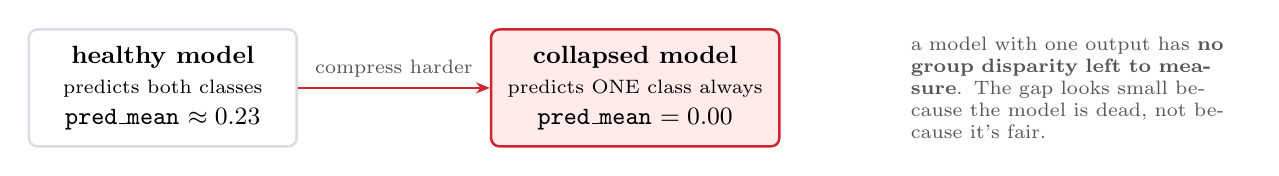
\begin{tikzpicture}[node distance=5mm]
\node[blk,minimum width=34mm,minimum height=12mm] (a) at (0,0)
  {\textbf{healthy model}\\\scriptsize predicts both classes\\\code{pred\_mean} $\approx 0.23$};
\node[blkb,minimum width=34mm,minimum height=12mm] (b) at (6.0,0)
  {\textbf{collapsed model}\\\scriptsize predicts ONE class always\\\code{pred\_mean} $= 0.00$};
\draw[arb] (a)--(b) node[midway,above,tiny] {compress harder};
\node[tiny,text width=42mm,align=left] at (11.6,0)
  {a model with one output has \textbf{no group disparity left to measure}.
   The gap looks small because the model is dead, not because it's fair.};
\end{tikzpicture}
\end{center}

\noindent Here's the real row from our data, at 80\% magnitude sparsity:

\begin{center}
\begin{tabular}{@{}lrrrrr@{}}
\toprule
 & \textbf{g0} & \textbf{g1} & \textbf{g2} & \textbf{g3} & \textbf{adj avg} \\
\midrule
accuracy & 100\% & 100\% & 0\% & 0\% & \textbf{76.8\%} \\
\bottomrule
\end{tabular}
\end{center}

\noindent That model predicts ``landbird'' for every single image. It gets 100\%
on both landbird groups and 0\% on both waterbird groups. And it still posts a
\textbf{76.8\% adjusted average}, which would look like a mediocre-but-working
model if you only read that one column.

That's why \code{pred\_mean} exists in the CSV. It's the average predicted class;
if it's pinned near 0 or 1, the model has collapsed. Those points get drawn
hollow in the figures and excluded from the trade-off plot.

\subsection{Head removal isn't monotonic, and that's fine}

You'd expect: remove more heads, get worse. Our data says removing \textbf{48}
heads scores \emph{better} on worst-group (34.1\%) than removing \textbf{36}
(1.1\%).

Two reasons, and neither is a bug:

\begin{itemize}[leftmargin=1.4em]
\item Ranking heads by weight size doesn't rank them by how much the model
actually \emph{uses} them. Cutting the ``smallest'' 36 can land worse than
cutting the smallest 48.
\item Near-collapse, which group is ``worst'' keeps reshuffling. At 36 heads the
worst group is waterbird-on-land; the numbers are bouncing around a nearly dead
model.
\end{itemize}

\noindent Treat the deep end of the head sweep as noise around a broken model,
not as signal. The honest finding lives at the shallow end: 6 heads out of 72
costing 22 points.

\subsection{Why the adjusted average, one more time}

This trips everyone up, so here it is as a picture:

\begin{center}
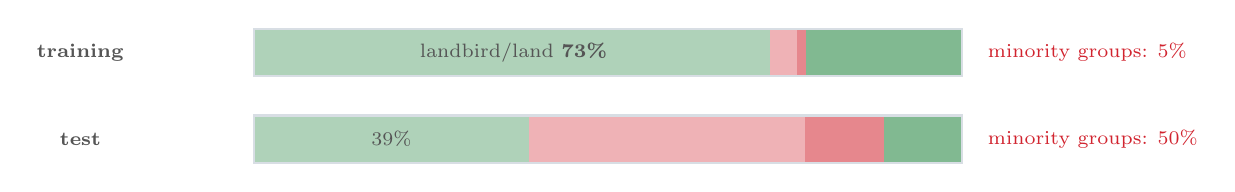
\begin{tikzpicture}
\node[tiny] at (-2.2,1.5) {\textbf{training}};
\node[tiny] at (-2.2,0.4) {\textbf{test}};
% training bar
\fill[good!35] (0,1.2) rectangle (6.56,1.8);
\fill[bad!35]  (6.56,1.2) rectangle (6.90,1.8);
\fill[bad!55]  (6.90,1.2) rectangle (7.01,1.8);
\fill[good!55] (7.01,1.2) rectangle (9.0,1.8);
\draw[rule,line width=0.8pt] (0,1.2) rectangle (9,1.8);
\node[tiny] at (3.3,1.5) {landbird/land \textbf{73\%}};
\node[tiny,anchor=west] at (9.2,1.5) {\textcolor{bad}{minority groups: 5\%}};
% test bar
\fill[good!35] (0,0.1) rectangle (3.5,0.7);
\fill[bad!35]  (3.5,0.1) rectangle (7.0,0.7);
\fill[bad!55]  (7.0,0.1) rectangle (8.0,0.7);
\fill[good!55] (8.0,0.1) rectangle (9.0,0.7);
\draw[rule,line width=0.8pt] (0,0.1) rectangle (9,0.7);
\node[tiny] at (1.75,0.4) {39\%};
\node[tiny,anchor=west] at (9.2,0.4) {\textcolor{bad}{minority groups: 50\%}};
\end{tikzpicture}
\end{center}

\noindent The test set is deliberately balanced; training isn't. A plain average
over the test set therefore over-weights rare groups relative to reality. The
adjusted average re-weights back to training proportions, which is the
convention in this research area. That's the only reason our headline is 98.2\%
instead of 91.7\% -- same model, same predictions, different weighting.

\subsection{The resume bug (a real one we found and fixed)}

Worth knowing because it's the kind of bug that produces \emph{no error at all}.

The sweep skips configurations already in the CSV. The check used to be
``have I seen this (method, value, granularity) before?''. Which is fine when
there's exactly one model.

\begin{center}
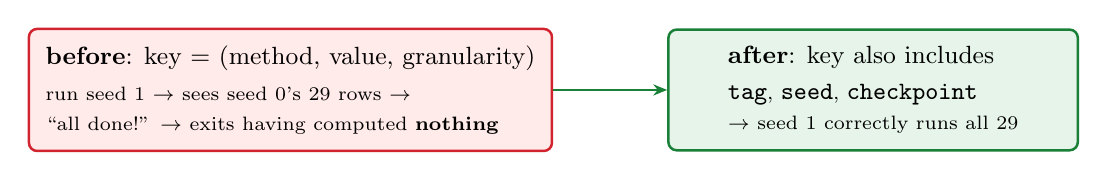
\begin{tikzpicture}[node distance=5mm]
\node[blkb,minimum width=52mm,minimum height=13mm,align=left] (a) at (0,0)
  {\textbf{before}: key $=$ (method, value, granularity)\\[2pt]
   \scriptsize run seed 1 $\to$ sees seed 0's 29 rows $\to$\\
   \scriptsize ``all done!'' $\to$ exits having computed \textbf{nothing}};
\node[blkg,minimum width=52mm,minimum height=13mm,align=left] (b) at (7.4,0)
  {\textbf{after}: key also includes\\[2pt]
   \scriptsize \code{tag}, \code{seed}, \code{checkpoint}\\
   \scriptsize $\to$ seed 1 correctly runs all 29};
\draw[arg] (a)--(b);
\end{tikzpicture}
\end{center}

\noindent The CSV would have looked complete and you'd have ``three seeds'' that
were actually one seed copied. Gate V12 now pins this down.

% ================================================================ PART 5
\section{Phase 2: can we fix it, and does the fix survive?}\label{sec:phase2}

\begin{note}{good}{Status: run, 3 seeds, and it worked}
Everything in this part has been executed. Headline: the fix takes worst-group
accuracy from \textbf{73.3\%} to \textbf{87.9\%}, and that gain survives gentle
compression but not heavy compression. Numbers below.
\end{note}

Phase 1 compressed a model that was never made robust in the first place. Fair
enough -- but a practitioner would say ``obviously, just fix the robustness
first''. Phase 2 does exactly that, and then asks the uncomfortable follow-up.

\begin{center}
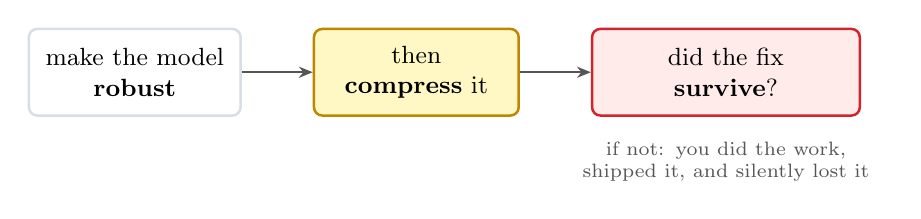
\begin{tikzpicture}[node distance=5mm]
\node[blk,minimum width=26mm,minimum height=11mm] (a) {make the model\\\textbf{robust}};
\node[blkw,minimum width=26mm,minimum height=11mm,right=9mm of a] (b) {then\\\textbf{compress} it};
\node[blkb,minimum width=34mm,minimum height=11mm,right=9mm of b] (c) {did the fix\\\textbf{survive}?};
\draw[ar] (a)--(b); \draw[ar] (b)--(c);
\node[tiny,below=2mm of c,text width=40mm,align=center]
  {if not: you did the work, shipped it, and silently lost it};
\end{tikzpicture}
\end{center}

\subsection{The fix: throw away the hardest training images}

This is from a 2025 paper (Mulchandani and Kim, ICLR). The idea is
counterintuitive and kind of beautiful:

\begin{note}{accent}{Why deleting data makes a model MORE robust}
A model takes the background shortcut because some training images are hard to
classify on their actual bird features. Where the real feature is hard, the easy
fake feature wins.

So: find the images the model finds hardest, delete them, and retrain. Without
those images pushing it toward the shortcut, the model has less reason to learn
``wet background $=$ waterbird''. You lose a bit of data and gain robustness.
\end{note}

\textbf{How ``hard'' is measured.} Train normally, stop at an early epoch, and
for each training image compute how far the model's predicted probabilities are
from the correct answer:
\[
  d_i \;=\; \bigl\lVert\, p(x_i) - \text{onehot}(y_i) \,\bigr\rVert_2
\]
Big $d_i$ means the model is confidently wrong or very unsure -- a hard image.

\begin{center}
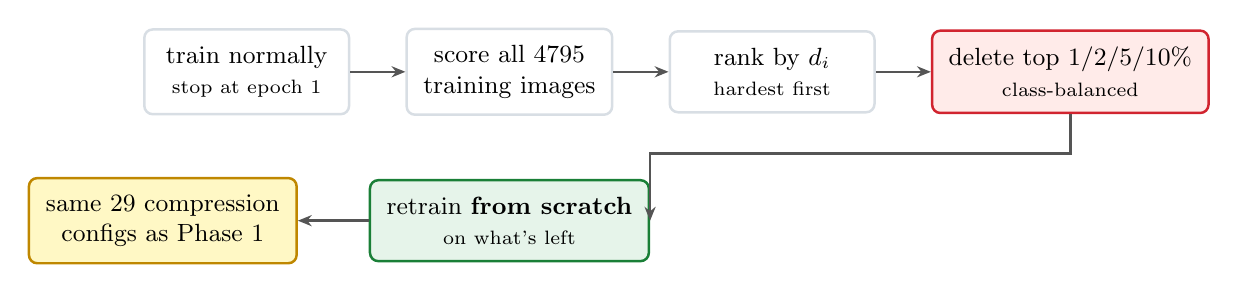
\begin{tikzpicture}[node distance=5mm]
\node[blk,minimum width=26mm,minimum height=10mm] (t) {train normally\\\scriptsize stop at epoch 1};
\node[blk,minimum width=26mm,minimum height=10mm,right=7mm of t] (s) {score all 4795\\training images};
\node[blk,minimum width=26mm,minimum height=10mm,right=7mm of s] (r) {rank by $d_i$\\\scriptsize hardest first};
\node[blkb,minimum width=28mm,minimum height=10mm,right=7mm of r] (d) {delete top 1/2/5/10\%\\\scriptsize class-balanced};
\draw[ar] (t)--(s); \draw[ar] (s)--(r); \draw[ar] (r)--(d);
\node[blkg,minimum width=34mm,minimum height=10mm,below=8mm of s] (rt) {retrain \textbf{from scratch}\\\scriptsize on what's left};
\draw[ar] (d.south) -- ++(0,-5mm) -| (rt.east);
\node[blkw,minimum width=34mm,minimum height=10mm,left=9mm of rt] (sw) {same 29 compression\\configs as Phase 1};
\draw[ar] (rt)--(sw);
\end{tikzpicture}
\end{center}

\subsection{We got this wrong the first time, and the wrong version is
instructive}

Our first attempt deleted the hardest images \emph{anywhere} in the training
set, without ever looking at which group they belonged to. That felt like the
honest thing to do -- a fix that needs group labels is a weaker fix. We ran it,
and worst-group accuracy got \emph{worse}, steadily worse the more we deleted.

Here is why, and it is obvious in hindsight. Think about which images a model
finds hardest. They are exactly the ones where the background lies: the water
bird standing on grass, the land bird over a lake. Those images are hard
\emph{because} the shortcut fails on them. So ``delete the hardest images''
quietly means ``delete the images that were holding the weak groups up''.

We measured it. The worst group has only 56 training images to begin with. At a
10\% deletion budget, the group-blind rule threw away \textbf{38 of those 56}:

\begin{center}\small
\begin{tabular}{@{}lrrrr@{}}
\toprule
& \multicolumn{4}{c}{share of each group deleted} \\
\cmidrule(l){2-5}
deletion budget & land/land (3498) & land/water (184) & \textbf{water/land (56)} & water/water (1057) \\
\midrule
1\%  & 0.3\% & 7.6\% & \textbf{14\%} & 1.5\% \\
2\%  & 0.6\% & 15\%  & \textbf{23\%} & 3.3\% \\
5\%  & 1.7\% & 33\%  & \textbf{45\%} & 9.0\% \\
10\% & 4.3\% & 48\%  & \textbf{68\%} & 19\%  \\
\bottomrule
\end{tabular}
\end{center}

\noindent And then we actually read the paper properly, and found it says this
itself. For a dataset like Waterbirds, where you \emph{can} tell which images
have the misleading background, the paper's method is told the groups and
deletes only from the groups the shortcut agrees with. It states plainly that
deleting the globally hardest images ``is not feasible'' here, for precisely the
reason our numbers show.

\begin{note}{accent}{The corrected rule, in one sentence}
Only consider images where the background \emph{agrees} with the bird -- the
easy, shortcut-confirming ones -- and delete the hardest of those. Never touch
the images where the background disagrees. Those are the ones teaching the model
to actually look at the bird.
\end{note}

So the project now has both versions, and keeps both:

\begin{itemize}[leftmargin=1.4em]
\item \f{--variant global} -- the group-blind rule. Kept because it demonstrates
the failure the paper warns about. Its results live in \code{old\_run\_Oct26/}.
\item \f{--variant spurious} -- the corrected rule. This is the one that
reproduces the paper, and the one all the numbers below come from.
\end{itemize}

\textbf{One more detail.} The corrected rule also levels up the two bird
classes, so that after deleting there are the same number of land birds as water
birds. Waterbirds starts badly lopsided (3682 against 1113), and that lopsidedness
is itself part of the problem. This is why the deletion budgets are so large --
25\%, 50\%, 75\% -- where the first attempt used 1--10\%. Most of that budget is
spent just evening up the two classes.

\subsection{The measurement: retention ratio}

Phase 2's headline number. Let $W_p$ and $W_e$ be \wg{} accuracy of the
\textbf{p}runed and \textbf{E}RM models at the same compression setting:

\[
  D(s) = W_p(s) - W_e(s) \qquad\qquad R(s) = \frac{D(s)}{D(0)}
\]

\noindent In words: $D(0)$ is how much robustness the fix bought you before any
compression. $D(s)$ is how much is left after compressing to level $s$. $R$ is
the fraction that survived. In the sketch below, the left arrow is $D(0)$ --
the gain the fix bought you -- and the right arrow is $D(s)$, however much of
it is still there after compressing.

\begin{center}
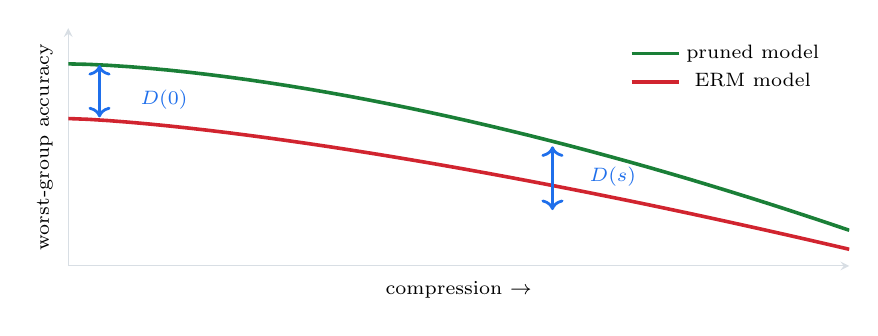
\begin{tikzpicture}
\begin{axis}[
  width=11.5cm, height=4.6cm,
  xlabel={compression $\to$}, ylabel={\wg{} accuracy},
  xlabel style={font=\scriptsize}, ylabel style={font=\scriptsize},
  xmin=0,xmax=1,ymin=0,ymax=1,
  xtick=\empty, ytick=\empty,
  axis lines=left, axis line style={draw=rule},
  legend style={font=\scriptsize,draw=none,at={(0.98,0.98)},anchor=north east},
]
\addplot[good,line width=1.3pt,domain=0:1,samples=40] {0.85-0.7*x^1.6};
\addlegendentry{pruned model}
\addplot[bad,line width=1.3pt,domain=0:1,samples=40] {0.62-0.55*x^1.4};
\addlegendentry{ERM model}
\draw[<->,accent,line width=1pt] (axis cs:0.04,0.845) -- (axis cs:0.04,0.625);
\node[font=\scriptsize,accent,anchor=west] at (axis cs:0.08,0.70) {$D(0)$};
\draw[<->,accent,line width=1pt] (axis cs:0.62,0.503) -- (axis cs:0.62,0.235);
\node[font=\scriptsize,accent,anchor=west] at (axis cs:0.655,0.375) {$D(s)$};
\end{axis}
\end{tikzpicture}
\end{center}

\begin{center}
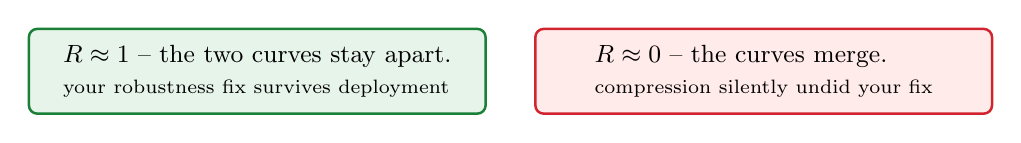
\begin{tikzpicture}[node distance=4mm]
\node[blkg,minimum width=58mm,minimum height=10mm,align=left] (r1)
  {$R \approx 1$ -- the two curves stay apart.\\\scriptsize your robustness fix survives deployment};
\node[blkb,minimum width=58mm,minimum height=10mm,right=6mm of r1,align=left] (r0)
  {$R \approx 0$ -- the curves merge.\\\scriptsize compression silently undid your fix};
\end{tikzpicture}
\end{center}

\subsection{The answers}

\textbf{Question one: does the fix work at all?} Yes, clearly, and at every
deletion budget we tried. All numbers are averages over 3 training runs.

\begin{center}\small
\begin{tabular}{@{}lrrr@{}}
\toprule
model & worst group & average & gain in worst group \\
\midrule
no fix (plain training) & 73.3\% & 98.3\% & --- \\
delete 25\% & 86.4\% & 94.7\% & \textbf{+13.1} \\
delete 50\% & \textbf{87.9\%} & 94.4\% & \textbf{+14.6} \\
delete 75\% & 87.3\% & 92.1\% & \textbf{+14.0} \\
\bottomrule
\end{tabular}
\end{center}

\noindent Two things to notice. The gain is roughly the same whichever budget
you pick, which is reassuring -- it means you don't have to tune the budget
carefully. And the average accuracy \emph{drops} by about 4 points while the
worst group gains 14. That trade is the entire point: you are deliberately
giving up a little overall accuracy to stop the model relying on backgrounds.
The paper reports the same shape of trade.

For reference, the paper gets 90.9\% worst group where we get 87.9\%. We are
about 3 points short, on a different model and a tenth of the training time.
Section~\ref{sec:shortfall} explains the gap honestly, because it is
interesting in itself.

\textbf{Question two -- the real one: does the fix survive compression?}

\begin{note}{accent}{The answer, and it is not what we first thought}
The fix survives compression right up to the point where compression has
wrecked the model \emph{for everybody}. Past that point the question stops
meaning anything.
\end{note}

Here is magnitude pruning, the gentlest of the four methods:

\begin{center}\small
\begin{tabular}{@{}lrrrl@{}}
\toprule
weights removed & no fix & with fix & $R$ & what it means \\
\midrule
none      & 73.3\% & 87.9\% & 1.00 & the fix bought 14.6 points \\
30\%      & 58.4\% & 81.9\% & \textbf{1.64} & still there, and wider than before \\
50\%      & 23.7\% & 53.0\% & \textbf{2.04} & still there \\
70\%      & 13.7\% & 13.4\% & $-0.15$ & gone -- both models are wrecked \\
\bottomrule
\end{tabular}
\end{center}

\noindent Read the 70\% row carefully, because it is easy to misread. $R$ went
to zero not because compression picked on the fix, but because at 70\% sparsity
\emph{neither} model works any more -- both are down near 13\%. $R$ is a ratio
of two gaps, and when both models are broken there is no gap left to measure in
either. A zero there means ``question no longer applies'', not ``fix destroyed''.

We checked this across all 195 settings that weren't collapsed, and it is the
cleanest result in the project:

\begin{center}\small
\begin{tabular}{@{}lrrr@{}}
\toprule
is the compressed model still usable? & settings & average $R$ & share with $R \ge 0.75$ \\
\midrule
yes -- worst group still above 40\% & 114 & \textbf{+1.30} & \textbf{96\%} \\
borderline -- 25\% to 40\%          & 14  & +1.30 & 86\% \\
no -- worst group below 25\%        & 67  & $-0.20$ & 13\% \\
\bottomrule
\end{tabular}
\end{center}

\noindent \textbf{If compression leaves a working model, the fix is still there
-- 96\% of the time, for all four compression methods.} If compression has
already destroyed the model, $R$ is noise. There is no middle ground and no
method that behaves specially.

\begin{note}{warn}{The mistake we nearly published}
Our first pass averaged $R$ within each compression method and got numbers like
``magnitude 1.26, FFN 0.31'', and we wrote down that compression harms the fix
differently depending on the method. That was wrong. Averaging $R$ over
compression levels smears a \textbf{$+2.04$ at 50\% sparsity} together with a
\textbf{$-0.15$ at 70\%} and produces a number describing neither.

The methods do differ, but in \emph{where the model dies}, not in whether the
fix survives: FFN-neuron removal kills it by 30\%, magnitude pruning survives to
50\%, per-channel quantization survives all the way down to 3 bits. That is
Phase~1's conclusion again -- the four methods are not interchangeable.

Lesson for reading any of this: \textbf{$R$ must always be read against a
compression level, never averaged over them.}
\end{note}

\subsection{Why we're 3 points short of the paper}\label{sec:shortfall}

Worth understanding, because it is a real limitation of the method rather than
a bug in our code.

The fix depends on ranking training images by how hard they are. That ranking is
only useful if the model hasn't learned the training set yet -- once it gets
nearly everything right, almost every image scores ``easy'' and the ranking
stops carrying information.

The paper trains a ResNet-50 for 100 epochs and scores after the first. Ours is
a pretrained vision transformer fine-tuned at a very low learning rate, and it
reaches \textbf{97.9\% training accuracy after two passes}. So by the time we
score, the ranking has already gone flat:

\begin{center}\small
\begin{tabular}{@{}lrr@{}}
\toprule
of the images our rule deletes & chosen on real difficulty & already near-perfect \\
\midrule
delete 25\% & 1080 & \textbf{2017 (65\%)} \\
delete 50\% & 1344 & \textbf{2281 (63\%)} \\
delete 75\% & 1479 & \textbf{2676 (64\%)} \\
\bottomrule
\end{tabular}
\end{center}

\noindent About two-thirds of what we delete are images the model already
classifies almost perfectly. The method's premise is ``delete the hard ones'',
and we are mostly deleting easy ones, because there aren't enough hard ones left
to fill the budget. What we're left doing is closer to ``shrink and balance the
training set'', which is itself a known way to help the weak groups -- hence we
still get most of the benefit, just not all of it.

That's a genuine finding about the method: \textbf{it needs a model that hasn't
yet fitted its training data.} In the transfer-learning setting most people
actually work in, that condition is easy to violate without noticing.

\subsection{Two things the code refuses to do}

\begin{itemize}[leftmargin=1.4em]
\item \textbf{It won't divide by noise.} If $D(0)$ is tiny -- meaning the data
pruning didn't actually help on our setup -- then $R = D(s)/D(0)$ would produce
enormous meaningless ratios out of rounding error. So there's a gate: if the
dense gain is below a threshold, $R$ is left \textbf{undefined} and the result is
reported as a null result. ``It didn't work'' is a real finding; a fabricated
ratio is not.

\item \textbf{It excludes collapsed models}, same as Phase 1. A dead model's
``retention'' is meaningless.
\end{itemize}

\subsection{One non-obvious engineering bit}

Scoring difficulty for seed 0 needs that seed's \emph{epoch-1} weights. But seed
0 is already trained and its checkpoint is what produced all the Phase 1
results. Retraining it would overwrite that file -- and training on Apple's GPU
isn't bit-for-bit reproducible, so the new checkpoint wouldn't be identical.
You'd silently decouple the published numbers from the weights behind them.

The fix is \code{--stop-after-epoch}: run the real schedule, stop early, write
\emph{no} checkpoint, keep only the scores. Costs 2 epochs instead of 10 and
touches nothing.


% ================================================================ PART 6
\section{How to actually read this code}

\subsection{A reading order that works}

\begin{enumerate}[leftmargin=1.6em]
\item \f{configs/base.yaml} -- 2 minutes. Now you know every knob.
\item \f{src/metrics.py} -- 10 minutes. Pure counting, no ML. Once
\code{group\_index} and \code{adjusted\_average} click, the results table reads
itself.
\item \f{src/evaluate.py} -- 5 minutes. 50 lines. This is what ``measuring the
model'' means here.
\item \f{src/compress/magnitude.py} -- 15 minutes. The simplest method, and the
tie-budget bit teaches you the mindset of the whole repo.
\item \f{src/sweep.py} -- 20 minutes. Now you see how it all gets driven.
\item Everything else, as needed.
\end{enumerate}

\subsection{The exercise that makes it stick}

Pick one number and chase it all the way through. Take \textbf{54.4\%} -- the
worst-group accuracy after 30\% magnitude pruning. Then:

\begin{center}
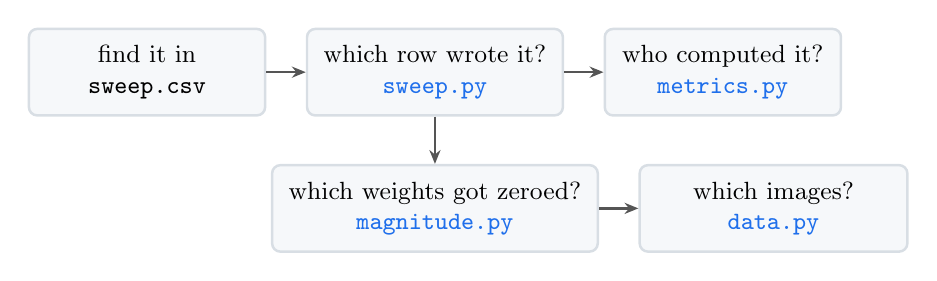
\begin{tikzpicture}[node distance=4mm]
\node[blkf,minimum width=30mm,minimum height=9mm] (a) {find it in\\\code{sweep.csv}};
\node[blkf,minimum width=30mm,minimum height=9mm,right=5mm of a] (b) {which row wrote it?\\\f{sweep.py}};
\node[blkf,minimum width=30mm,minimum height=9mm,right=5mm of b] (c) {who computed it?\\\f{metrics.py}};
\node[blkf,minimum width=34mm,minimum height=9mm,below=6mm of b] (d) {which weights got zeroed?\\\f{magnitude.py}};
\node[blkf,minimum width=34mm,minimum height=9mm,right=5mm of d] (e) {which images?\\\f{data.py}};
\draw[ar] (a)--(b); \draw[ar] (b)--(c);
\draw[ar] (b.south) -- ++(0,-3mm) -| (d.north);
\draw[ar] (d)--(e);
\end{tikzpicture}
\end{center}

\noindent Takes about half an hour and after it you'll know this codebase better
than most people know code they wrote themselves.

\subsection{Commands you'll actually use}

\begin{center}
\begin{tabular}{@{}ll@{}}
\toprule
\textbf{Command} & \textbf{What it does} \\
\midrule
\code{pytest tests/ -q} & run all 52 gates ($\sim$35s) \\
\code{python -m src.figures} & rebuild the three figures from the CSV \\
\code{python -m src.sweep --seed 0} & re-run the sweep (resumes if interrupted) \\
\code{./run\_phase2.sh} & the whole Phase 2 pipeline \\
\code{caffeinate -i <cmd>} & stop the Mac sleeping mid-run \\
\bottomrule
\end{tabular}
\end{center}

\begin{note}{warn}{One practical gotcha}
This machine is set to sleep after 1 minute idle. A sleeping Mac is why one
training epoch in the Phase 1 log took \textbf{3338 seconds} when the others took
\textbf{114}. Always prefix long runs with \code{caffeinate -i}, keep the lid
open, and stay on mains power.
\end{note}

\subsection{The three things to remember}

\begin{enumerate}[leftmargin=1.6em]
\item \textbf{Average accuracy hides group damage.} 0.5 points vs 14.9 points,
from the same operation.
\item \textbf{Structured compression hurts more than it looks.} 6 attention
heads out of 72 cost 18 points of worst-group accuracy.
\item \textbf{A collapsed model can look fine.} A model that predicts one class
for every image has no gap between its groups at all. Always check
\code{pred\_mean} before believing a small gap.
\item \textbf{The fix works, and it survives compression until compression
breaks the model outright.} Worst group 73.3\% $\to$ 87.9\%, and that gain is
still there 96\% of the time in any setting where the compressed model is still
usable.
\item \textbf{Never average a ratio over compression levels.} Doing that is how
we briefly convinced ourselves of a conclusion that wasn't there.
\end{enumerate}

\bigskip
\begin{center}
{\color{ink2}\small Built from the repo as it stands. Both phases are run, over
3 seeds.\\ Phase 1 is in \code{results/sweep.csv}; Phase 2 in
\code{results/sweep\_spur*.csv} and \code{results/retention\_*.csv}.\\
The first, failed Phase 2 attempt is kept in \code{old\_run\_Oct26/}.}
\end{center}

\end{document}
